

\begin{center}
	\section*{Questões José Guilherme - Nota 02}
\end{center}

\begin{flushleft}

1. Assuma que existam apenas dois bens e suponha que o preço do bem 2 aumentou. Represente graficamente essa mudança. Se sabemos que o consumidor exaure toda a sua renda e prefere consumir mais a menos, esse aumento do preço do bem 2 irá afetar o seu bem-estar de que forma? Isso ocorrerá sempre? \singlespacing

\textbf{Resposta:} breezzj


\begin{center}
\textbf{Gráfico demonstrando o exercício.} 
\singlespacing
\begin{tikzpicture}[scale=0.5, axis/.style={very thick, ->, >=stealth'}, important line/.style={thick}, dashed line/.style={dashed, thin}, pile/.style={thick, ->, >=stealth', shorten <=2pt, shorten >=2pt}, every node/.style={color=black}]

			% Eixos (axis)
		\draw[axis] (0,0)  -- (11.5,0) node(xline)[right] {$x1$};
		\draw[axis] (0,0) -- (0,11.5) node(yline)[above] {$x2$};

			% Declaração dos pontos
		\coordinate (A) at (0,10);
		\coordinate (B) at (10,0);

			% Linhas do gráfico
		          \draw [thick] (0,8) -- (8,0);
		          \draw [thick] (0,8) -- (6,0);
		          \node [left] at (0,8){$\dfrac{m}{\textit{p2}}$};
		          \node [below] at (8,0) {$\dfrac{m}{\textit{p1}}$};
                  \node [below] at (6,0) {$\dfrac{m}{\textit{p1}'}$};
                   \node [right] at (4,3) {$\swarrow$};
                 

\end{tikzpicture}    
\singlespacing

\end{center}
Suponhamos, que temosz dois bens $\textit{a}$ e $\textit{b}$, temos, uma representação normal do consumo destes dois bens, quando o preço do bem $\textit{b'}$ aumenta, logo, sabemos que o agente irá consumir menos, pois, a sua renda $\textit{m}$ não é infinita, logo, ocorre uma rotação na inclinação, conforme demonstrado no gráfico. Ou seja, esse aumento gera perda de bem-estar, afinal, o consumidor não irá consumir $\textit{b}$, e verá o seu consumo diminui para $\textit{b'}$. Porém, nem sempre pode ocorrer perda de bem-estar, se houvesse aumenta do consumo do bem $\textit{a}$, ocorreria uma situação adversa. \singlespacing

2. Suponha que os preços de todos os bens aumentem na mesma proporção. Isso é equivalente a uma mudança na renda? Explique.
\singlespacing
\textbf{Resposta:} Depende, por exemplo, ocorre uma mudança na renda, já que que a alteração dos preços provoca uma diminuição do poder que a renda tem ao consumidor, dobrando os preços da restrição, ocorre essa variação da renda. \textbf{Por exemplo:}

\begin{center}

A restrição orçamentária: $\textit{p1x1} + \textit{p2x2} +...+ \textit{pnxn} \leq \textit{m}$ \singlespacing

Quando ocorre um aumento simultâneo em todos os preços (respeitando a condição de "ceteris paribus":  $\textit{(2p1)x1} + \textit{(2p2)x2} +...+ \textit{(2pn)xn} \leq \textit{(m)}$ \singlespacing

\end{center}

 \singlespacing

3. Suponha que o bem 1 teve o seu preço quadruplicado e o bem 2 teve o seu preço duplicado. O que ocorre com a inclinação da reta orçamentária? Faz sentido dizermos que o bem 1 se tornou relativamente mais barato do que o bem 2? \singlespacing

\textbf{Resposta:} 
\\
\begin{center}
\textbf{Gráfico demonstrando o exercício.} 
\singlespacing
\begin{tikzpicture}[scale=0.5, axis/.style={very thick, ->, >=stealth'}, important line/.style={thick}, dashed line/.style={dashed, thin}, pile/.style={thick, ->, >=stealth', shorten <=2pt, shorten >=2pt}, every node/.style={color=black}]

			% Eixos (axis)
		\draw[axis] (0,0)  -- (11.5,0) node(xline)[right] {$x1$};
		\draw[axis] (0,0) -- (0,11.5) node(yline)[above] {$x2$};

			% Declaração dos pontos
		\coordinate (A) at (0,10);
		\coordinate (B) at (10,0);

			% Linhas do gráfico
		          \draw [thick] (0,8) -- (8,0);
		          \draw [thick] (0,8) -- (6,0);
		          \node [left] at (0,8){$\dfrac{m}{\textit{a}}$};
		          \node [below] at (8,0) {$\dfrac{m}{\textit{b}'}$};
                  \node [below] at (6,0) {$\dfrac{m}{\textit{b}}$};
                  \node [right] at (3.6,3) {$\nearrow$};
                 

\end{tikzpicture}    
\singlespacing

\end{center}

Em tese, sim. Porque o bem 1 ou $\textit{a}$ teve um aumento quadruplicado, já o bem 2 ou $\textit{b}$ teve um aumento, porém, um aumento menor que o bem 1, logo, ele se tornou barato em relação ao bem $\textit{a}$, mas ainda houve um aumento, no gráfico acima, fizemos a mudança de inclinação demonstrando o aumento do consumo do bem 2. \singlespacing

{$x_{1}+2(x_{2}-5)+5=10$}, se {$x_{2}>5$}, {$0\leq$}{$x_{1}$}{$\leq5$}\\
{$2(x_{1}-5)+5+x_{2}=10$}, se {$x_{1}>5$}, {$0\leq$}{$x_{2}$}{$\leq5$}\\



4. Suponha que o individuo consome apenas dois bens, em que o bem 1 é saúde, medido emtermos qualidade (ou seja, quanto mais afastado da origem no eixo horizontal, melhor o serviço de saúde adquirido). O governo resolve prover gratuitamente o nível de saúde $\textit{x1}$ = Ā(e apenas esse nível é provido de modo gratuito). Represente a reta orçamentária neste caso. \singlespacing

\textbf{Respostas:} \singlespacing
\begin{center}
\textbf{Gráfico demonstrando o exercício.} 
\singlespacing
\begin{tikzpicture}[scale=0.5, axis/.style={very thick, ->, >=stealth'}, important line/.style={thick}, dashed line/.style={dashed, thin}, pile/.style={thick, ->, >=stealth', shorten <=2pt, shorten >=2pt}, every node/.style={color=black}]

			% Eixos (axis)
		\draw[axis] (0,0)  -- (11.5,0) node(xline)[right] {$x1$};
		\draw[axis] (0,0) -- (0,11.5) node(yline)[above] {$x2$};

			% Declaração dos pontos
		\coordinate (A) at (0,10);
		\coordinate (B) at (10,0);

			% Linhas do gráfico
		          \draw [thick] (0,8) -- (8,0);
		          
					\draw[dashed] (4,4) -- (4,0);
                    \draw[dashed] (4,4) -- (0,4);
          	
                     \node [left] at (0,8){$\dfrac{m}{\textit{a}}$};
		          \node [below] at (8,0) {$\dfrac{m}{\textit{b}}$};
                  \node [below] at (4,0){$\textit{x1}$ = Ā};
                  \draw[fill] (4,4) circle [radius =0.06];


                 

\end{tikzpicture}    
\singlespacing

\end{center}

Neste caso, havera uma quebra da restrição orçamentária, pois a uma inferencia do governo para que a saúde seja gratuita, no ponto $\textit{x1}$ = Ā, logo, a restrição orçamentária não funcionará normalmente, ocasionando essa quebra. \singlespacing

5. Ilustre graficamente a restrição orçamentária para o caso de três bens. O que ocorre com essa restrição se a renda aumentar? E se o preço de um bem aumentar? \singlespacing

\textbf{Respostas:} 
\\
Primeiro, para demonstrar a variação do aumenta da renda, pegamos o bem x$\textit{2}$ e aplicamos a variação na renda, ou seja, havendo um aumento na renda, ocorre uma variação no consumo do bem x$\textit{2}$, havendo um aumento na quantidade consumida em \textbf{m} para \textbf{m'}. Já no caso do bem x$\textit{1}$, ocorre o inverso, quando o preço do bem aumenta, ocorrendo uma diminuição na quantidade consumida \textbf{b} para \textbf{b'}.

\begin{center}

\tdplotsetmaincoords{70}{110}     
\begin{tikzpicture}[scale=1.5,tdplot_main_coords]      
\draw[thick,black,->] (0,0,0) -- (5,0,0) node[anchor=north east]{$x\textit{1}$};       
\draw[thick,black,->] (0,0,0) -- (0,5,0) node[anchor=north west]{$x\textit{2}$};       
\draw[thick,black,->] (0,0,0) -- (0,0,3) node[anchor=south]{$x\textit{3}$};   

		          \draw [thick] (0,0,2) -- (2,0,0);
		          \draw [thick] (0,0,2) -- (1,0,0);
		          \draw [thick] (0,0,2) -- (0,1,0);
		          \draw [thick] (2,0,0) -- (0,1,0);
		          

		          \node [left] at (0,0,2){$\dfrac{m}{\textit{a}}$};
		          \node [below] at (2,0,0) {$\dfrac{m}{\textit{b}}$};
		          \node [below] at (1,0,0) {$\dfrac{m}{\textit{b'}}$};
                   \node [left] at (0.4,0,0.1) {$\nearrow$};
					\node [below] at (0,1,0) {$\dfrac{m'}{\textit{c}}$};
					\node [right] at (0,1.2,0,6) {$\rightarrow$};


     
       
\end{tikzpicture}        
\end{center}

6. Suponha que existam apenas dois bens e o governo resolve controlar os preços desses bens do seguinte modo: o preço é R\$ 1,00 até 5 unidades adquiridas, e o preço é R\$ 2,00 para unidades adicionais (acima das primeiras 5 unidades adquiridas). Suponha que Carlos tem uma renda de R\$ 10,00. \singlespacing

\textbf{A}) Ilustre graficamente a reta orçamentária de Carlos.

\textbf{Resposta:}
\\
\textbf{A)}
\begin{center}
				\begin{tikzpicture}[scale=1] 
						
					\draw[->, very thick] (-0.1,0) -- (8,0) node[right]{$x_1$}; 
					\draw[->, very thick] (0,-0.1) -- (0,8) node[above]{$x_2$};
					\draw (0,7) -- (7,0) node[below]{$7,5$}; 
					\node[left] at (0,7){$7,5$};
					\draw[dashed] (3,4) -- (3,0);
                    \draw[dashed] (3,4) -- (0,4);
                    \node[below] at (3,0){$5$};
                    \node[left] at (0,4){$5$};
                    
					\end{tikzpicture}
					
					
\end{center}

\textbf{B)}
\\
\begin{center}

{$x_{1}+2(x_{2}-5)+5=10$}, se {$x_{2}>5$}, {$0\leq$}{$x_{1}$}{$\leq5$}\\
{$2(x_{1}-5)+5+x_{2}=10$}, se {$x_{1}>5$}, {$0\leq$}{$x_{2}$}{$\leq5$}
\end{center}

7. Suponha uma economia com dois bens, denotados por x e y. A reta orçamentária de Maria é $p_{x}^{M}\textit{x}$ + $p_{y}^{M}\textit{y} = m^{M}$ é a reta orçamentária de João $p_{x}^{j}\textit{x}$ + $p_{y}^{j}\textit{y}$ = $m^{j}$, onde $p_{x}^{M}$/$p_{y}^{M}$ $\neq$ $p_{x}^{j}$/$p_{y}^{j}$. Ou seja, o custo de mercado entre x e y para Maria é diferente do custo de mercado para João. Maria e João decidem se casar e formar uma família onde a renda dos dois é gasta em conjunto, apesar de que os preços dos bens para cada um deles continuam os mesmos de antes.  \singlespacing

\textbf{A)} Defina a restrição orçamentária do casal.
\\
\textbf{B)} Haverá especialização na compra dos bens? \singlespacing

\textbf{Resposta:} 
\\
\textbf{A)} 
\\
\begin{center}

{$p_{x}x$} + {$p_{y}y$} = $m$.
\\

\textbf{Onde:}
\\
$p_{x}$ = min{$\lbrace$}{$p^M_x$},{$p^J_x$}{$\rbrace$},\\
$p_{y}$ = min{$\lbrace$}{$p^M_y$},{$p^J_y$}{$\rbrace$},\\
{$m$} = {$m^M$} e {$m^J$}.\\
\end{center}

\textbf{B)}
\\
Sim, haverá especialização pois, a Maria irá concentrar renda no produto mais barato no caso o produto x. Enquanto, o João irá comprar bens y, assim, realizando uma especialização na compra dos produtos. \singlespacing

8. Dados p\textit{1} = -1; p\textit{2} = -2 e m = 16, pede-se:
\singlespacing
\textbf{A)} Desenhe a restrição orçamentária;
\\
\textbf{B)} Qual o valor da declividade da restrição orçamentária?
\\
\textbf{C)} Se o consumidor resolve gastar tudo em q1, qual a quantidade que pode comprar de q1?
\\
\textbf{D)} Idem para q2;
\\
\textbf{E)} Suponha que a renda aumente para 20. Desenhe a nova restrição orçamentária;
\\
\textbf{F)} Qual o valor da declividade da nova restrição orçamentária?
\\
\textbf{G)} Suponha que p1 aumente para 2 e p2 e m = 16. Desenhe a nova restrição orçamentária e o valor da sua declividade.

\singlespacing

\textbf{Resposta:} \singlespacing

\textbf{A)}
\\
\begin{center}

A primeira restrição é formada pelo $\dfrac{M}{p\textit{1}} = \dfrac{16}{1}$ = 16. 
\singlespacing
Já a segunda é composta por $\dfrac{M}{p\textit{2}} = \dfrac{16}{2}$ = 8.

\begin{tikzpicture}[scale=0.5, axis/.style={very thick, ->, >=stealth'}, important line/.style={thick}, dashed line/.style={dashed, thin}, pile/.style={thick, ->, >=stealth', shorten <=2pt, shorten >=2pt}, every node/.style={color=black}]

			% Eixos (axis)
		\draw[axis] (0,0)  -- (11.5,0) node(xline)[right] {$x1$};
		\draw[axis] (0,0) -- (0,11.5) node(yline)[above] {$x2$};

			% Declaração dos pontos
		\coordinate (A) at (0,10);
		\coordinate (B) at (10,0);

			% Linhas do gráfico
		          \draw [thick] (0,8) -- (8,0);
		          \node [below] at (8,0){$16$};
		          \node [left] at (0,8) {$8$};
            
                 

\end{tikzpicture}    
\end{center}


\textbf{B)}
\\
O valor da declividade da RO é $\dfrac{-p\textit{1}}{p\textit{2}}$, usando os valores $p\textit{1}$ = 1 e $p\textit{2}$ = 2, calculamos que $\dfrac{1}{2}$, o resultado da nossa inclinação é -0,5.
\singlespacing

\textbf{C)}
\\
Se ele gastar tudo em q$_{1}$, ele poderá consumir a quantidade de 16. Já que ficaria dessa seguinte forma: $\dfrac{M}{p\textit{1}} = \dfrac{16}{1}$ = 16. 
\singlespacing

\textbf{D)}
\\
Se gastar tudo em $q_{2}$, a quantidade que será consumida será de $\dfrac{M}{p\textit{2}} = \dfrac{16}{2}$ = 8.
\singlespacing

\textbf{E)}
\\
\begin{center}

A primeira restrição é formada pelo $\dfrac{M}{p\textit{1}} = \dfrac{20}{1}$ = 20. 
\singlespacing
Já a segunda é composta por $\dfrac{M}{p\textit{2}} = \dfrac{20}{2}$ = 10.

\begin{tikzpicture}[scale=0.5, axis/.style={very thick, ->, >=stealth'}, important line/.style={thick}, dashed line/.style={dashed, thin}, pile/.style={thick, ->, >=stealth', shorten <=2pt, shorten >=2pt}, every node/.style={color=black}]

			% Eixos (axis)
		\draw[axis] (0,0)  -- (11.5,0) node(xline)[right] {$x1$};
		\draw[axis] (0,0) -- (0,11.5) node(yline)[above] {$x2$};

			% Declaração dos pontos
		\coordinate (A) at (0,10);
		\coordinate (B) at (10,0);

			% Linhas do gráfico
		          \draw [thick] (0,8) -- (8,0);
		          \node [below] at (8,0){$20$};
		          \node [left] at (0,8) {$10$};
            
                 

\end{tikzpicture}    
\end{center}
\singlespacing

\textbf{F)}
\\
Continuará a mesma, pois para se calcular a declividade é dividindo os preços.
\singlespacing

\textbf{G)}

\begin{center}

A primeira restrição é formada pelo $\dfrac{M}{p\textit{1}} = \dfrac{16}{2}$ = 8. 
\singlespacing
Já a segunda é composta por $\dfrac{M}{p\textit{2}} = \dfrac{16}{2}$ = 8.

\begin{tikzpicture}[scale=0.5, axis/.style={very thick, ->, >=stealth'}, important line/.style={thick}, dashed line/.style={dashed, thin}, pile/.style={thick, ->, >=stealth', shorten <=2pt, shorten >=2pt}, every node/.style={color=black}]

			% Eixos (axis)
		\draw[axis] (0,0)  -- (11.5,0) node(xline)[right] {$x1$};
		\draw[axis] (0,0) -- (0,11.5) node(yline)[above] {$x2$};

			% Declaração dos pontos
		\coordinate (A) at (0,10);
		\coordinate (B) at (10,0);

			% Linhas do gráfico
		          \draw [thick] (0,8) -- (8,0);
		          \node [below] at (8,0){$8$};
		          \node [left] at (0,8) {$8$};
            
                 

\end{tikzpicture}    
\end{center}

A declividade será de 1, pois $\dfrac{-p_{1}}{p_{2}}$, terá o resultado de $\dfrac{-2}{2}$ gerando o resultado de 1.
\singlespacing


9. Imagine que haja apenas duas mercadorias: energia elétrica e outros bens. A mercadoria "outros bens" tem um preço de R\$ 1 por unidade, os primeiros 1000kWh de energia elétrica consumidos no período de um mês têm o preço de R\$ 0,50 por kWh; a energia elétrica que for consumida em excesso a 1.000 kWh/mês é vendida ao preço de R\$ 2. Desenhe a curva de restrição orçamentária de um consumidor que tem uma renda mensal igual a R\$ 1.000,00.
\textbf{Resposta:}
\begin{center}
				\begin{tikzpicture}[scale=1] 
						
					\draw[->, very thick] (-0.1,0) -- (8,0) node[right]{Outros Bens}; 
					\draw[->, very thick] (0,-0.1) -- (0,8) node[left]{Energia Elétrica};
					\draw (0,6) -- (6,0) node[below]{$10.000$}; 
					\node[left] at (0,6){$5.750$};
					\draw[dashed] (5,1) -- (5,0);
					\node[below] at (4.7,0){$9.500$};
                    \draw[dashed] (5,1) -- (0,1);
                    \node[left] at (0,1){$1.000$};

                    
					\end{tikzpicture}
					
					
\end{center}


10. Imagine que m = 100, $p_{1}$ = -1, e $p_{2}$ = 2.

\singlespacing
\textbf{A)} Faça o gráfico da restrição orçamentária;
\\
\textbf{B)} O que acontece com a restrição se os preços e a renda subirem em uma mesma proporção?
\\
\textbf{C)} Desenhe a nova restrição se a renda cair pela metade e o preço do bem dois também cair pela metade.
\singlespacing
\textbf{Resposta:}
\\
\textbf{A)} 
\\
$p_{1}$ = -1, e $p_{2}$ = 2 e a renda m = 100.
\singlespacing
logo, $\dfrac{m}{p_{1}}$ e $\dfrac{m}{p_{2}}$, usando os preços na formula, temos, $\dfrac{100}{1}$ = 100 e $\dfrac{100}{2}$ = 50.


\begin{center}

\begin{tikzpicture}[scale=0.5, axis/.style={very thick, ->, >=stealth'}, important line/.style={thick}, dashed line/.style={dashed, thin}, pile/.style={thick, ->, >=stealth', shorten <=2pt, shorten >=2pt}, every node/.style={color=black}]

			% Eixos (axis)
		\draw[axis] (0,0)  -- (11.5,0) node(xline)[right] {$x1$};
		\draw[axis] (0,0) -- (0,11.5) node(yline)[above] {$x2$};

			% Declaração dos pontos
		\coordinate (A) at (0,10);
		\coordinate (B) at (10,0);

			% Linhas do gráfico
		          \draw [thick] (0,8) -- (8,0);
		          \node [below] at (8,0){$100$};
		          \node [left] at (0,8) {$50$};
            
                 

\end{tikzpicture}    
\end{center}
\singlespacing
\textbf{B)}
\\
 Acontece uma ilusão monetária, já que os preços e a renda terão o mesmo aumento da renda, logo, um efeito nulo, apenas haverá mudanças nos valores e não no poder de compra do consumidor.
\singlespacing

\textbf{C)}
\\
$p_{1}$ = -0,5, e $p_{2}$ = 1 e a renda m = 100.
\singlespacing
logo, $\dfrac{m}{p_{1}}$ e $\dfrac{m}{p_{2}}$, usando os preços na formula, temos, $\dfrac{50}{1}$ = 50 e $\dfrac{50}{1}$ = 50. 

\begin{center}

\begin{tikzpicture}[scale=0.5, axis/.style={very thick, ->, >=stealth'}, important line/.style={thick}, dashed line/.style={dashed, thin}, pile/.style={thick, ->, >=stealth', shorten <=2pt, shorten >=2pt}, every node/.style={color=black}]

			% Eixos (axis)
		\draw[axis] (0,0)  -- (11.5,0) node(xline)[right] {$x1$};
		\draw[axis] (0,0) -- (0,11.5) node(yline)[above] {$x2$};

			% Declaração dos pontos
		\coordinate (A) at (0,10);
		\coordinate (B) at (10,0);

			% Linhas do gráfico
		          \draw [thick] (0,8) -- (8,0);
		          \node [below] at (8,0){$50$};
		          \node [left] at (0,8) {$50$};
            
                 

\end{tikzpicture}    
\end{center}

\begin{center}
	\section*{Questões José Guilherme - Nota 03}
\end{center}

\subparagraph{}
\textbf{2} - O técnico de vôlei Bernardo acha que os jogadores devem ter três qualidade: altura, agilidade e obediência. Se o jogador A é melhor que o jogador B em duas dessas três características, então Bernardo prefere A a B. Para os outros casos, ele é indiferente entre A e B. Carlos mede 2,08m, é pouco ágil e obediente. Luis mede 1,90m, é muito ágil, e muito desobediente. Paulo mede 1,85m, é ágil, e extremamente obediente.
\singlespacing

\textbf{A)} Bernardo prefere Carlos ou Luis? Bernardo prefere Luis ou Paulo? Bernardo prefere Carlos ou Paulo?
\\
\textbf{B)} As preferências do técnico são transitivas?
\\
\textbf{C)} Depois de perder vários campeonatos, Bernardo decide mudar sua forma de comparar os jogadores. Agora ele prefere o jogador A ao jogador B se A é melhor do que B nas três caracteristicas. Ele é indiferente entre A e B se eles têm todas as três caracteristicas iguais. Para todas as outras possibilidades, Bernardo diz que não é possível comparar os jogadores. As novas preferências de Bernardo são: completas? transitivas? reflexivas? Justifique.

\singlespacing

\textbf{Respostas:}
\\
\textbf{A)} Na primeira opção, Bernardo vai agir da seguinte maneira Carlos $\succeq$ Luis, já que Carlos respeita a condição de ter duas qualidades. Na segunda opção, entre Luis $\succeq$  Paulo vai ocorrer uma preferência, pois, Luis é mais alto e com mais agilidade. Já Paulo $\succeq$ Carlos, pois, Paulo tem qualidades melhores que Carlos. \singlespacing

\textbf{B)} Não são transitivas, pois, na última escolha entre Paulo e Carlos, deveria ser o inverso para respeitar a  regra de transitividade.
\singlespacing

\textbf{C)} \singlespacing



\textbf{5} Desenhe as curvas de indiferença para as seguintes utilidades:\\


\paragraph{}a) Utilidade Linear: u{$(x_1,x_2)$} = {$ax_1 + bx_2$}, a,b {$>$} 0.\\


\textbf{Resposta:}\\

\begin{center} %Centralização do gráfico a ser desenhado
				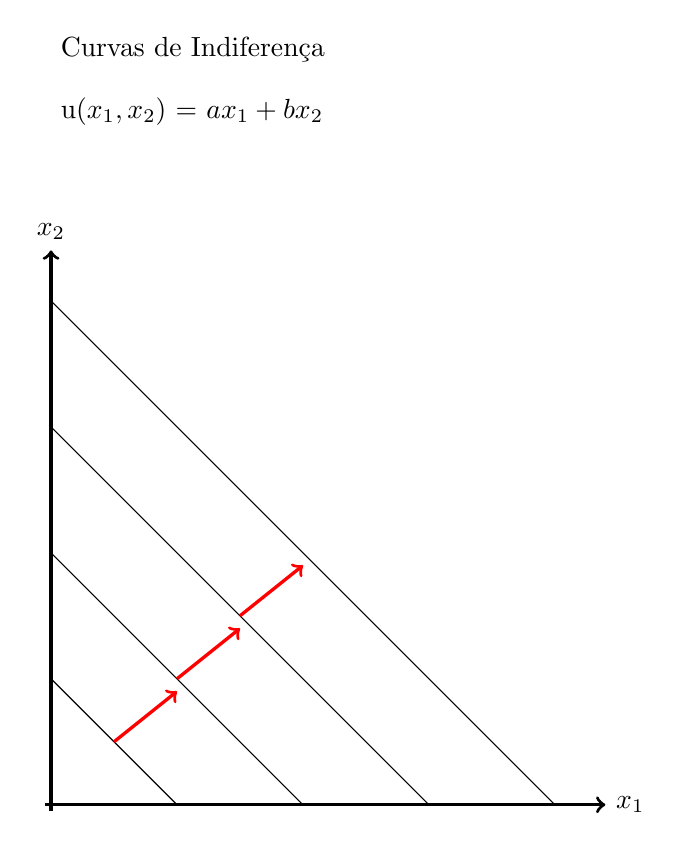
\begin{tikzpicture}[scale=0.8] %Início do desenho e definição da escala
						%Eixos
					\draw[->, very thick] (-0.1,0) -- (8.8,0) node[right]{$x_1$}; %Eixo X1
					\draw[->, very thick] (0,-0.1) -- (0,8.8) node[above]{$x_2$}; %Eixo X2
						%Retas
					\draw (0,8) -- (8,0);
					\draw (0,6) -- (6,0);
					\draw (0,4) -- (4,0);
					\draw (0,2) -- (2,0);
					\draw (0,12) node [right] {Curvas de Indiferença};
					\draw (0,11) node [right] {u{$(x_1,x_2)$} = {$ax_1 + bx_2$}};
					\draw[->, very thick, red] (1,1) -- (2,1.8); 
					\draw[->, very thick, red] (2,2) -- (3,2.8);
			        \draw[->, very thick, red] (3,3) -- (4,3.8);
					
				\end{tikzpicture}\\
				 
			\end{center} 


\paragraph{} b)  Utilidade de Leontief: u{$(x_1,x_2)$} = {$min \{ax_1,bx_2\}$}, a, b {$>$} 0.\\

\textbf{Resposta:}\\

\begin{center} %Centralização do gráfico a ser desenhado
				\begin{tikzpicture}[scale=0.8] %Início do desenho e definição da escala
						%Eixos
					\draw[->, very thick] (-0.1,0) -- (8.8,0) node[right]{$x_1$}; %Eixo X1
					\draw[->, very thick] (0,-0.1) -- (0,8.8) node[above]{$x_2$}; %Eixo X2
						%Retas
					
					\draw (1.5,2) -- (7,2);
					\draw (1.5,2) -- (1.5,7);
					
					\draw (2.5,3) -- (7,3);
					\draw (2.5,3) -- (2.5,7);
				
				    \draw (3.5,4) -- (7,4);
					\draw (3.5,4) -- (3.5,7);
					
					
					\draw[->, very thick, red] (3,2.5) -- (3.5,2.9); 
					\draw[->, very thick, red] (1.7,5.2) -- (2.2,5.5); 
					
					\draw[->, very thick, red] (4,3.5) -- (4.5,3.9); 
					\draw[->, very thick, red] (2.7,5.2) -- (3.2,5.5);
					
					\draw (0,12) node [right] {Curvas de Indiferença};
					\draw (0,11) node [right] {u{$(x_1,x_2)$} = min{$\{ax_1, bx_2\}$}};
				\end{tikzpicture}\\
				
				 
			\end{center} 
			
			
\paragraph{} c) Utilidades com um Bem Neutro: u{$(x_1, x_2)$} = {$x_1$} e u{$(x_1, x_2)$} = {$x_2$}.

\textbf{Resposta:}\\

\begin{center} %Centralização do gráfico a ser desenhado
				\begin{tikzpicture}[scale=0.8] %Início do desenho e definição da escala
						%Eixos
					\draw[->, very thick] (-0.1,0) -- (8.8,0) node[right]{$x_1$}; %Eixo X1
					\draw[->, very thick] (0,-0.1) -- (0,8.8) node[above]{$x_2$}; %Eixo X2
						%Retas
					\draw (1.7,0) -- (1.7,4);
					\draw (2.8,0) -- (2.8,4);
					\draw (3.9,0) -- (3.9,4);
					\draw (0,12) node [right] {Curvas de Indiferença};
					\draw (0,11) node [right] {u{$(x_1, x_2)$} = {$x_1$}};
					
				\end{tikzpicture}\\
				 
			\end{center} 
 

\begin{center} %Centralização do gráfico a ser desenhado
				\begin{tikzpicture}[scale=0.8] %Início do desenho e definição da escala
						%Eixos
					\draw[->, very thick] (-0.1,0) -- (8.8,0) node[right]{$x_1$}; %Eixo X1
					\draw[->, very thick] (0,-0.1) -- (0,8.8) node[above]{$x_2$}; %Eixo X2
						%Retas
					\draw (0,1.7) -- (4,1.7);
					\draw (0,2.8) -- (4,2.8);
					\draw (0,3.9) -- (4,3.9);
					\draw (0,12) node [right] {Curvas de Indiferença};
					\draw (0,11) node [right] {u{$(x_1, x_2)$} = {$x_2$}};
					
				\end{tikzpicture}\\
				 
			\end{center} 
			
\paragraph{} d) Utilidade com um Mal: u{$(x_1, x_2)$} = {$x_1 - x_2$}.\\

\textbf{Resposta:}\\

\begin{center} %Centralização do gráfico a ser desenhado
				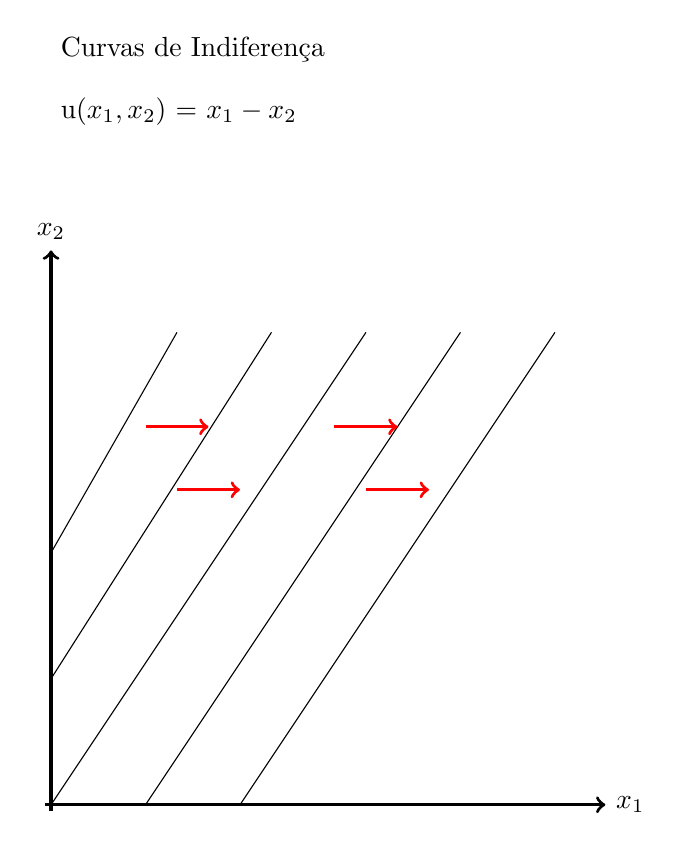
\begin{tikzpicture}[scale=0.8] %Início do desenho e definição da escala
						%Eixos
					\draw[->, very thick] (-0.1,0) -- (8.8,0) node[right]{$x_1$}; %Eixo X1
					\draw[->, very thick] (0,-0.1) -- (0,8.8) node[above]{$x_2$}; %Eixo X2
					
					\draw (0,4) -- (2,7.5);
					\draw (0,2) -- (3.5,7.5);
					\draw (0,0) -- (5,7.5);
					\draw (1.5,0) -- (6.5,7.5);
					\draw (3,0) -- (8,7.5);
                	\draw[->, very thick, red] (1.5,6) -- (2.5,6);
                	\draw[->, very thick, red] (2,5) -- (3,5);
				    \draw[->, very thick, red] (4.5,6) -- (5.5,6);
				    \draw[->, very thick, red] (5,5) -- (6,5);
				    \draw (0,12) node [right] {Curvas de Indiferença};
					\draw (0,11) node [right] {u{$(x_1, x_2)$} = {$x_1 - x_2$}};
					
					
					\end{tikzpicture}\\
				 
			\end{center}

\singlespacing

\textbf{Questões ANPEC}

1. Um consumidor possui a função de utilidade cardinal dada por $U(x_1,x_2)=x_1 x_2$. As preferências do consumidor são convexas. (Questão ANPEC - 2OO3)
\singlespacing

\textbf{Resposta:}

Sim, essa função de utilidade é do tipo Cobb-Douglas, logo, as utilidades que fazem parte deste grupo são convexas.

\begin{center}

\begin{tikzpicture}[scale=0.6]

\draw[thick,<->] (0,10) node[above]{$y$}--(0,0)--(10,0) node[right]{$x$};
\node [right] at (1,8.5) {$x_{1}$};


\draw(1,8)--(8,1) ;


\draw(1,8.5) to [out=280,in=175](8.5,1) node[right]{$x_{2}$};



\end{tikzpicture}
\\
\textbf{Gráfico:} Convexidade Estrita
\end{center}
\singlespacing

2 - A figura abaixo mostra as curvas de indiferença de um consumidor e a direção na qual a utilidade deste
consumidor aumenta.
\\
1- Existe saciedade.
\\
\begin{center}
\begin{tikzpicture}[scale=1]
			% Axis			
			\draw [->] (0,0) node [below] {0} -- (0,0) -- (5.5,0) node [below] {$x_1$};
			\draw [->] (0,0) node [below] {0} -- (0,0) -- (0,5.5) node [above] {$x_2$};
			
			% Indifference curve
			\draw (0,0) to [in=-175,out=-280] (4,4.5);
			\draw (2,0) to [in=-175,out=-280] (5,2.8);
			\draw[->] (3,2) -- (2,3);
			\end{tikzpicture}
			\end{center}
			\label{anpect2004_consumidor}
\begin{itemize}

\item[2)] Considerando a Figura acima, o indivíduo gosta da diversificação.
		\item[3)] Considerando a Figura acima, o bem $x_1$ é indesejável;
		\item[4)] Considerando a Figura acima, no equilíbrio, o indivíduo só consome um tipo de bem.
		\item[5)] Considerando a Figura acima, a utilidade marginal do bem 2 é não negativa.
		\end{itemize}

\textbf{Respostas:}
\\
1- Não existe saciedade, primeiro, porque essa curva de indiferença tem um formato pouco usual, já que a TMS é crescente. Também ocorrerá que o eixo $x_2$ irá atigir o seu máximo enquanto o $x_1$ será igual a 0.
\singlespacing
2- Isso também não é verdade, já que o agente economico está querendo maximar o bem $x_2$, o que ocorre neste caso é que as suas preferências não são convexas quando o individuo está diversificando o seu consumo, o padrão dessa utilidade é concava, fazendo o inverso dessa operação.
\singlespacing
3- Sim, a figura do eixo $x_1$ é considerado um bem "mal".
\singlespacing
4- Sim, o individuo irá se concentrar em consumir apenas a mercadoria 2.
\singlespacing


\begin{center}
	\section*{Questões José Guilherme - Nota 04}
\end{center}
\singlespacing

\textbf{Questão 2:} Suponha uma função utilidade definida por:

\begin{center}
	$U(x_{1}, y_{2})$ = min$\lbrace{x_{2} + 2x_{1},x_{1} + 2x_{2} }\rbrace$

\end{center}

\textbf{a)} Desenha a curva de indiferença para $U(x_{1}, y_{2})$ = 20.
\singlespacing
\textbf{b)} Para que os valores de $p_{1}$/$p_{2}$ a solução ótima consistirá em $x_{1}$ = 0 e $x_{2}$ = m/$p_{2}$?
\singlespacing
\textbf{c)} Para que os valores de $p_{1}$/$p_{2}$ a solução ótima consistirá em $x_{1}$ = m/$p_{1}$ e $x_{2}$ = 0? 
\singlespacing
\textbf{d)} Para que os valores de $p_{1}$/$p_{2}$ a solução ótima será interior (ou seja, $x_{1}^{*} >0$ e $x_{2}^{*}>0$)?
\singlespacing

\textbf{Respostas:}
\singlespacing

\textbf{a)} \\
	Algumas condições para a solução da questão \textbf{a};
	\singlespacing
	1 - Complementaridade.
	\singlespacing
	   \begin{equation} \label{eq:1}
		\left\{
		\begin{array}{ll}
		x_{2} + 2x_{1} \\
		x_{1} + 2x_{2}
		\end{array}
		\right.
		\end{equation}
\\
		\begin{center}
			Desenvolvendo:
		\end{center}


	\begin{equation}
	\left\{
	\begin{array}{ccc}
	x_{2} + 2x_{1} = & 0 \\
	x_{1} + 2x_{2} = & 0 \\
	x_{1} = x{2} 
	\end{array}
	\right.
	\end{equation}

	\begin{equation}
		\left\{
		\begin{array}{ll}
		x_{2} = - 2x_{1} \\
		x_{1} = - 2x_{2}
		\end{array}
		\right.
		\end{equation}\\

   Sabendo que estamos trabalhando com substitutos e complementares, vamos agora, a segunda condição.
   \singlespacing
   2- Restrição.
   \\
   $$m = P_{1}x_{1} + P_{2}x_{2}$$ 
   \singlespacing

   3- Aplicando o metódo para solucionar os problemas de uma questão complementar.
		
			$$U(x_{1}, y_{2}) = 20$$ \\
		\begin{center}
			
		logo, \\
		\end{center}

		\begin{equation} \label{eq:2}
		{x_{2} + 2x_{1} = 20} 
		\end{equation}

		\begin{equation}
			{x_{1} + 2x_{2} = 20} \label{eq:3}
		\end{equation}
		\begin{center}
			\textbf{Substituindo} (3) na equação(4).
		\end{center}
		
		\begin{equation} \label{eq:4}
		{x_{2} + 2(-2x_{2}) = 20}
		\end{equation}
		
		\begin{equation} \label{eq:5}
			{x_{2} = \dfrac{20}{3}}
		\end{equation}
		
		\begin{center}
			logo, \\
		\end{center}
		
		\begin{equation}
			x_{1} = x{2} 
		\end{equation}

		\begin{equation}
			x_{1} = \dfrac{20}{3} $$\\$$
			x_{2} = \dfrac{20}{3}
		\end{equation}

		\begin{center}
	
		\textbf{Gráfico}
		\end{center}

		\begin{center} %Centralização do gráfico a ser desenhado
			\begin{tikzpicture}[scale=0.8] %Início do desenho e definição da escala
				%Desenho dos eixos
				\draw[->, very thick] (-0.1,0) -- (8,0) node[right]{$x_1$}; 
				\draw[->, very thick] (0,-0.1) -- (0,8) node[above]{$x_2$};

				%Desenho das retas
				\draw (0,7) -- (2.5,2) -- (6,0) node[below]{$20$}; 
				\draw[dashed] (2.5,2) -- (2.5,0);
				\draw[dashed] (2.5,2) -- (0,2);
				\node[left] at (0,7){$20$};
				\node[below] at (2.5,0){$\dfrac{20}{3}$};
				\node[left] at (0,2){$\dfrac{20}{3}$};
				\draw[->, very thick, black] (0.6,5.8) -- (1,6.8); 
				\draw[->, very thick, black] (2.3,2) -- (4,2.5); 
				\draw[->, very thick, black] (4.2,1) -- (5.3,1); 
				\draw[->, very thick, black] (1.5,4) -- (2.5,4); 
				\draw (0.9,7) node [right] {curva de indiferença $\overline{u} = 20 $};
				\draw (4,2.5) node [right]  {$x_{1} = x_{2}$};
				\draw (2.5,4) node [right]  {$x_{2} > x_{1}$};
				\draw (5.5,1) node [right]  {$x_{1} > x_{2}$};
			\end{tikzpicture}\\
			
			 
		\end{center} 
   
		\textbf{b)}
		
		Sabendo como se aplica a resolução dos substitutos perfeitos e complementares, vamos ter que pensar da seguinte maneira;
		\\
		\begin{equation} 
			x_{1}^{m}(p_{1}, p_{2}, m) = \left\{
			\begin{array}{l}
			x_{1} + 2x_{2}
			\end{array}
			\right.
			\end{equation}
		\singlespacing

		\textbf{Questão 5:} Encontre as demandas ótimas para os seguitnes casos, onde $\alpha > 0$ e $\beta >0$.
		\singlespacing

		\textbf{b)} $u=(x_{1, x_{2}}) = x_{1}^{\frac{\alpha}{\alpha + \beta}} x_{2}^{\frac{\beta}{\alpha + \beta}}$;
		
		\singlespacing



		\textbf{Resposta:} 
		\singlespacing

		$$u=(x_{1, x_{2}}) = x_{1}^{\frac{\alpha}{\alpha + \beta}} x_{2}^{\frac{\beta}{\alpha + \beta}} \rightarrow P_{1}x_{1}+P_{2}x_{2} = m$$
		\\
		$$\ell= x_{1}^{\frac{\alpha}{\alpha + \beta}} x_{2}^{\frac{\beta}{\alpha + \beta}} - P_{1}x_{1}\lambda -P_{2}x_{2}\lambda  + m\lambda $$

		\begin{equation}
			\frac{\partial\ell}{\partial x_{1}} = \dfrac{\alpha}{\alpha + \beta}x_{1}^{-\frac{\alpha}{\alpha + \beta}} x_{2}^{\frac{\beta}{\alpha + \beta}} - P_{1}\lambda = 0 $$\\$$
			\lambda = \dfrac{\dfrac{\alpha}{\alpha + \beta}x_{1}^{-\frac{\alpha}{\alpha + \beta}} x_{2}^{\frac{\beta}{\alpha + \beta}}}{P_{1}}
		\end{equation}
\\
		\begin{equation}
		\frac{\partial\ell}{\partial x_{2}} = \dfrac{\beta}{\alpha + \beta}x_{1}^{\frac{\alpha}{\alpha + \beta}} x_{2}^{-\frac{\beta}{\alpha + \beta}} - P_{2}\lambda = 0 
		$$\\$$
		\lambda = \dfrac{\dfrac{\beta}{\alpha + \beta}x_{1}^{\frac{\alpha}{\alpha + \beta}} x_{2}^{-\frac{\beta}{\alpha + \beta}}}{P_{2}}
		\end{equation}
\\
\begin{center}
	Igualando os $\lambda = \lambda$ \\
\end{center}
		\begin{equation}
		\dfrac{\dfrac{\alpha}{\alpha + \beta}x_{1}^{-\frac{\alpha}{\alpha + \beta}} x_{2}^{\frac{\beta}{\alpha + \beta}}}{P_{1}} = \dfrac{\dfrac{\beta}{\alpha + \beta}x_{1}^{\frac{\alpha}{\alpha + \beta}} x_{2}^{-\frac{\beta}{\alpha + \beta}}}{P_{2}} 
		$$\\$$
		\dfrac{\dfrac{\alpha}{\alpha + \beta} x_{2}^{\frac{\beta}{\alpha + \beta}}}{P_{1}x_{1}^{\frac{\alpha}{\alpha + \beta}}} = \dfrac{\dfrac{\beta}{\alpha + \beta} x_{1}^{\frac{\alpha}{\alpha + \beta}}}{P_{2}x_{2}^{\frac{\beta}{\alpha + \beta}}}
		\end{equation}
\\

	\begin{center}
	Isolando o $x_{2}$, temos o resultado:
	\end{center}

	\begin{equation}
		x_{2} = \dfrac{\beta}{\alpha}\dfrac{P_{1}x_{1}}{P_{2}}
	\end{equation}
\\

	\begin{center}
		Derivando em função de $\lambda$ e Substituindo por $x_{2}$ \\
	\end{center}

	\begin{equation}
		\frac{\partial\ell}{\partial \lambda} = -P_{1}x_{1} - P_{2}x_{2} + m = 0 
		$$\\$$
		-P_{1}x_{1} - P_{2}\dfrac{P_{1}}{P_{2}}\dfrac{\beta x_{1}}{\alpha} + m = 0
		$$\\$$
		m = P_{1}x_{1} - \dfrac{P_{1}{\beta x_{1}}}{\alpha} 
		$$\\$$
		x_{1} = \dfrac{\alpha}{(\alpha + \beta)}.\dfrac{m}{P_{1}}
	\end{equation}
	\\
	\begin{center}
		Por fim, substituindo $x_{1}$ em $x_{2}$.
	\end{center}

	\begin{equation}
		x_{2} = \dfrac{\beta}{\alpha}\dfrac{P_{1}x_{1}}{P_{2}}
		$$\\$$
		x_{2} = \dfrac{\beta}{(\alpha + \beta)}.\dfrac{m}{P_{2}}
	\end{equation}
\singlespacing

\begin{center}
	\section*{Questões José Guilherme - Nota 05}
\end{center}
\singlespacing
\textbf{1-} Considere a seguinte função de utilidade:
\\

	$$u(x_{1},x_{2}) = x_{1}^{0,5} + x_{2}^{0,5}.$$

\textbf{a)} Determine as funções de demanda marshallianas e a função de utilidade indireta.
\singlespacing
\textbf{b)} Mostre que a função de utilidade indireta satisfaz as propriedades de homogeneidade de grau 0 nos preços e na renda.
\singlespacing
\textbf{Respostas:}
\\
\textbf{a)}
\singlespacing

\begin{equation}
	u(x_{1},x_{2}) = x_{1}^{0,5} + x_{2}^{0,5}  \ s.a \ [p_{1}x_{1} + p_{2}x_{2} - m] $$\\$$
	\ell = x_{1}^{0,5} + x_{2}^{0,5} - \lambda (p_{1}x_{1} + p_{2}x_{2} - m) $$\\$$
	\frac{\partial\ell}{\partial x_{1}} = 0,5x_{1}^{0,5} - \lambda p_{1} = 0
	$$\\$$
	\frac{\partial\ell}{\partial x_{2}} = 0,5x_{2}^{0,5} - \lambda p_{2} = 0
	$$\\$$
	\frac{\partial\ell}{\lambda} = p_{1}x_{1} - p_{2}x_{2} - m = 0
\end{equation}
\singlespacing
\begin{center}
	
Agora dividindo a primeira CPO pela segunda, teremos:
\end{center}

\begin{equation}
	\left( \frac{x_{2}}{x_{1}} \right)^{0,5} = \frac{p_{1}}{p_{2}}
\end{equation}

\begin{center}
	Agora, isolando o $x_{2}$:

\end{center}

\begin{equation}
	x_{2} = \left( \frac{p_{2}}{p_{1}} \right)^{2}x_{1}
\end{equation}

\begin{center}
	Substituindo na restrição orçamentária:
\end{center}

\begin{equation}
	-p_{1}x_{1} - p_{2} \left( \frac{p_{1}^{2}}{p_{2}}\right)x_{1} = -m
	$$\\$$
	-p_{1}x_{1} - \left( \frac{p_{2}p_{1}^{2}x_{1}}{p_{2}} \right) = -m (-1)
	$$\\$$
	x_{1}\left( \frac{p_{1}^{2} + p_{1}p_{2}}{p_{2}} \right) = m
	$$\\$$
	x_{1}\left(\frac{p_{1}p_{2} + p_{1}^{2}}{p_{2}}\right) = m
	$$\\$$
	x_{1} = \frac{p_{2}m}{p_{1}p_{2} + p_{1}^{2}}
\end{equation}

\begin{center}
	Agora substituindo $x_{1}$ em $x_{2}$.
\end{center}

\begin{equation}
	x_{2} = \left( \frac{p_{2}}{p_{1}} \right)^{2}x_{1}
	$$\\$$
	x_{2} = \left( \frac{p_{1}}{p_{2}} \right)^{2}.\left( \frac{p_{2}m}{p_{2}p_{1} + p_{1}^{2}} \right)
	$$\\$$
	x_{2} = \frac{p_{1}m}{p_{1}p_{2} + p_{2}^{2}}
\end{equation}

\begin{center}
	Agora, a função utilidade indireta é quando você pega as funções $x_{1}$ e $x_{2}$ e substitui na função utilidade.
\end{center}

\begin{equation}
	u(x_{1},x_{2}) = x_{1}^{0,5} + x_{2}^{0,5}
	$$\\$$
	v(p_{1},p_{2},m) = \left[ \left( \dfrac{p_{2}m}{p_{1}p_{2} + p_{1}^{2}} \right)^{0,5} + \left( \frac{p_{1}m}{p_{1}p_{2} + p_{2}^{2}} \right)^{0,5}  \right] 
	$$\\$$
	v(p_{1},p_{2},m) = \left[ \left( \dfrac{p_{2}}{p_{1}p_{2} + p_{1}^{2}} \right)^{0,5} + \left( \frac{p_{1}}{p_{1}p_{2} + p_{2}^{2}} \right)^{0,5}  \right] \sqrt{m}
\end{equation}
\singlespacing
\textbf{b)}
	\begin{center}
		Agora multiplicando todos os termos por t, iremos provar a homogeneidadede grau 0.
	\end{center}

	\begin{equation}
		v(p_{1},p_{2},m) = \left[ \left( \dfrac{p_{2}}{p_{1}p_{2} + p_{1}^{2}} \right)^{0,5} + \left( \frac{p_{1}}{p_{1}p_{2} + p_{2}^{2}} \right)^{0,5}  \right] \sqrt{m}
		$$\\$$
		v(tp_{1},tp_{2},tm) = \left[ \left( \dfrac{(tp_{2})}{(tp_{1})(tp_{2}) + (tp_{1}^{2})} \right)^{0,5} + \left( \frac{(tp_{1})}{(tp_{1})(tp_{2}) + (tp_{2})^{2}} \right)^{0,5}  \right] \sqrt{tm}
		$$\\$$
		v(tp_{1},tp_{2},tm) = \dfrac{1}{\sqrt{t}} \left[ \left( \dfrac{p_{2}}{(p_{1})(p_{2}) + (p_{1}^{2})} \right)^{0,5} + \left( \frac{p_{1}}{(p_{1})(p_{2}) + (p_{2})^{2}} \right)^{0,5}  \right] \sqrt{t}\sqrt{m} 
		$$\\$$
		v(p_{1},p_{2},m) = \left[ \left( \dfrac{p_{2}}{p_{1}p_{2} + p_{1}^{2}} \right)^{0,5} + \left( \frac{p_{1}}{p_{1}p_{2} + p_{2}^{2}} \right)^{0,5}  \right] \sqrt{m}
	\end{equation}
\singlespacing

	\textbf{2-} Suponha que a utilidade de Rafael seja u($x_{1},x_{2}$) = $x_{1}^{0,2}x_{2}^{0,8}$, onde $x_{1}$ é a quantidade de alimentos que Rafael consome e $x_{2}$ é a quantidade de todos os outros bens que Rafael consome (um bem composto, portanto). Suponha que o preço do bem 2 é $p_{2}$ = R\$ 1 e que a renda de Rafael é R\$ 1.000.
	\singlespacing

	\textbf{a)} Se o preço do bem 1 é R\$ 2, qual é o consumo de alimentos do Rafael?
	\singlespacing

	\textbf{d)} Construa um diagrama comparando as situações $\textbf{b)}$ e $\textbf{c)}$ e mostre em qual situação o consumidor está melhor.

	\singlespacing

	\textbf{Respostas:}

	\singlespacing
	
	\textbf{a)} 
	\singlespacing

	\begin{center}
		
		Primeiro passo é achar as demandas de $x_{1}$ e $x_{2}$.

	\end{center}

	\begin{equation}
		u(x_{1},x_{2}) = x_{1}^{0,2}x_{2}^{0,8} \ s.a \ (p_{1}x_{1} + p_{2}x_{2} - m)
		$$\\$$
		\ell = x_{1}^{0,2}x_{2}^{0,8} - \lambda(p_{1}x_{1} + p_{2}x_{2} - m)
		$$\\$$
		\ell = x_{1}^{0,2}x_{2}^{0,8} -\lambda p_{1}x_{1} - \lambda p_{2}x_{2} + \lambda m $$\\$$
		\frac{\partial\ell}{\partial x_{1}} = 0,2x_{1}^{-0,8} - \lambda p_{1} = 0
		$$\\$$
		\frac{\partial\ell}{\partial x_{2}} = 0,8x_{2}^{-0,2} - \lambda p_{2} = 0
		$$\\$$
		\frac{\partial\ell}{\partial \lambda } = -p_{1}x_{1} - p_{2}x_{2} + m = 0
		$$\\$$
		\lambda = \dfrac{0,2x_{1}^{-0,8}x_{2}^{0,8}}{p_{1}}
		$$\\$$
		\lambda = \dfrac{0,8x_{1}^{0,2}x_{2}^{-0,2}}{p_{2}}
	\end{equation}
	
	\begin{center}
		Agora, devemos igualar os $\lambda$ = $\lambda$.
	\end{center}

	\begin{equation}
		\dfrac{0,2x_{2}^{0,8}}{p_{1}x_{1}^{0,8}} = \dfrac{0,8x_{1}^{0,2}}{p_{2}x_{2}^{0,2}}
		$$\\$$
		0,2p_{2}x_{2} = 0,8p_{1}x_{1}
		$$\\$$
		x_{2} = \dfrac{0,8p_{1}x_{1}}{0,2p_{2}} \rightarrow x_{2} = \dfrac{4p_{1}x_{1}}{p_{2}}
	\end{equation}

	\begin{center}
		Substituindo $x_{2}$ na terceira CPO.
	\end{center}

	\begin{equation}
		-p_{1}x_{1} - p_{2}x_{2} + m =0 \rightarrow -p_{1}x_{1} - p_{2}x_{2} = -m
		$$\\$$
		-p_{1}x_{1} - p_{2}\left( \dfrac{4p_{1}x_{1}}{p_{2}} \right) = -m
		$$\\$$
		x_{1} = \dfrac{m}{5p_{1}}
	\end{equation}

	\begin{center}
		substituindo $x_{1}$ em $x_{2}$.
	\end{center}

	\begin{equation}
		x_{1} = \dfrac{m}{5p_{1}}
		$$\\$$
		x_{2} = \dfrac{4p_{1}x_{1}} {p_{2}}
		$$\\$$
		x_{2} = \dfrac{4p_{x1}}{p_{2}}.\dfrac{m}{5p_{1}} 
		$$\\$$
		x_{2} = \dfrac{4m}{5p_{2}}
	\end{equation}

	\begin{center}
		Agora que temos as funções demanda, o preço e a renda, podemos substituir e obter os resultados.
	\end{center}

	\begin{equation}
		x_{1} = \dfrac{m}{5p_{1}}
		$$\\$$
		x_{1} = \dfrac{1000}{5.2}
		$$\\$$
		x_{1} = 100
		$$\\$$
		x_{2} = \dfrac{4m}{5p_{2}}
		$$\\$$
		x_{2} = \dfrac{4.1000}{5.1}
		$$\\$$
		x_{2} = 800
	\end{equation}
	
	\textbf{d)}
	\\
\begin{center}
	Situação \textbf{b}: $p_{1} = 4, p_{2} = 1 \ e \ m = 1000$
\end{center}

\begin{equation}
	x_{1} = \dfrac{m}{5p_{1}}
	$$\\$$
	x_{2} = \dfrac{4m}{5p_{2}} 
	$$\\$$
	x_{1} = \dfrac{1000}{5.4}
	$$\\$$
	x_{1} = 50
	$$\\$$
	x_{2} = \dfrac{4.1000}{5.1}
	$$\\$$
	x_{2} = 800
\end{equation}

\begin{center}
	É o que ocorre na questão \textbf{b}, quando o preço duplica. Agora no caso \textbf{c} quando o governo deseja subsidiar o bem 1, temos que ter as noçoes de que $p_{1} = 2, p_{2} = 1 \ e \ m = 1000.$
\end{center}

\begin{equation}
	\overline{m} = m - tx_{1}
	$$\\$$
	\overline{m} = 1000 - 2.100
	$$\\$$
	\overline{m} = 1000 - 200 \rightarrow \overline{m} = 800
	$$\\$$
	x_{1} = \dfrac{800}{5.2} \rightarrow x_{1} = 80
	$$\\$$
	x_{2} = \dfrac{4.800}{5.1} \rightarrow x_{2} = 640
\end{equation}
 \begin{center}
	 Agora, temos as nossas quantidades consumidas pra $x_{1}$ e $x_{2}$. Por fim, vamos fazer uma comparação para saber em qual situação o consumidor estará melhor, se é com ou sem subsídio.
 \end{center}
 \begin{equation}
	\rightarrow u(x_{1}^{*}u_{2}^{*}) = 50^{0,2}800^{0,8} = 459,48.
	$$\\$$
	\rightarrow u(x_{1}^{**}u_{2}^{**}) = 80^{0,2}640^{0,8} = 422,24.
 \end{equation}

 \begin{center}
	 Ou seja, se pegar a utilidade sem subsídio será 459,48 e com subsídio será de 422,24. ocorrendo que autilidade sem subsídio é melhor do que com essa política.
 \end{center}
\singlespacing

\begin{center}
	\section*{Questões José Guilherme - Nota 06}
\end{center}

\singlespacing

\textbf{1-} Derive as agregações de Engel e Cournot para o caso de \textit{n} bens. Reescreva essas agregações em termos de elasticidades. Interprete (por exemplo, é possível que todos os bens que um individuo consuma sejam bens inferiores? Por quê? Se um individuo consome \textit{n} bens, no máximo quantos bens podem ser inferiores? Justifique sua resposta).

\singlespacing

\textbf{Respostas:}

\singlespacing

Derivando a Lei de Walras para \textit{n} bens:

\begin{equation}
	p_{1}x_{1}(\textbf{p},m) + p_{2}x_{2}(\textbf{p},m) + \ldots + p_{n}x_{n}(\textbf{p},m) = m
\end{equation}
\\
Quando derivamos em relação a renda, obteremos o seguinte resultado:

\begin{equation}
	p_{1}\dfrac{\partial x_{1}(\textbf{p},m)}{\partial m} + p_{2}\dfrac{\partial x_{2} (\textbf{p},m)}{\partial m} + \ldots + p_{n}\dfrac{\partial x_{n} (\textbf{p}, m)}{\partial m} = 1
\end{equation}

Agregação de Engel:

\begin{equation}
	\dfrac{p_{1}x_{1}}{m} \left(\dfrac{m}{x_{1}} \dfrac{\partial x_{1}}{\partial m} \right) + 	\dfrac{p_{2}x_{2}}{m} \left(\dfrac{m}{x_{2}} \dfrac{\partial x_{2}}{\partial m} \right) + \ldots + 	\dfrac{p_{n}x_{n}}{m} \left(\dfrac{m}{x_{n}} \dfrac{\partial x_{n}}{\partial m} \right) = 1
\end{equation}

A agregação de Engel escrita em termos de elasticidades:

\begin{equation}
	s_{1}n_{1} + s_{2}n_{2} + \ldots + s_{n}n_{n} = 1
\end{equation}

Para derivar a lei de Walras e encontrar a agregação de Cournot, precisamos usar o caso geral.

\begin{equation}
	x_{i}^{m} + \sum_{k=1}^{n} \dfrac{\partial x_{k}^{m}}{\partial p_{i}} = 0
\end{equation}

Agora derivando em relação ao preço do bem i:

\begin{equation}
	x_{i}(\textbf{p}, m) + \sum_{j=1}^{n}p_{j} \dfrac{\partial x_{j}(\textbf{p}, m)}{\partial p_{i}} = 0 
	$$\\$$
	\dfrac{x_{i}p_{i}}{m} + \sum_{j=1}^{n}p_{j} \dfrac{p_{j}x_{j}}{m}\dfrac{p_{i}}{x_{j}} \dfrac{\partial x_{j}}{\partial p_{i}}
	$$\\$$
	0 = s_{i} + \sum_{j=1}^{n}p_{j} s_{j} \in_{ji}^{m}
	$$\\$$
	s_{i}(1 + \in_{ii}^{m}) = - \sum_{j=1, j\neq i}^{n} s_{j} \in_{ji}^{m}
\end{equation}

Para o caso da agregação de Engel, no máximo n - 1 bens podem ser inferiores (se todos os bens forem inferiores, então a elasticidade-renda $n_{i}$ será negativa para todo bem $_{i}$ = 1,2,$\ldots$, n. Como se $s_{i}$ $\geq$ 0 ($s_{i}$ é a fração da renda gasta com bem $_{i}$), então se todas elasticidades-renda forem negativas, a igualdade acima não será verificada). Logo, não será possível gastar toda a sua renda com bens inferiores, haverá de ter pelo menos um bem normal.
\\
No caso da agregação de Cournot, Se o bem $_{i}$ é elástico (inelástico), então $\in_{ii}^{m}$ $<$ -1, e o lado esquerdo é negativo (positivo). O lado direito deve ser negativo (positivo) também, ou seja, a soma ponderada das
elasticidades-preço cruzadas dos outros bens com relação ao bem $_{i}$ deve ser na média positiva(negativa). Portanto, se a demanda do bem i é elástica (inelástica), então os outros bens devem ser, na média ponderada pela fração gasta em cada bem, substitutos (complementares)do bem i, independente de como esses bens afetem a função de utilidade.
\\
Outra implicação que pode ser tirada da equação é a relação dos gastos nos outros bens devido a uma mudança no preço do bem $_{i}$: essa relação depende da elasticidade-preço de $_{i}$. Se a demanda do bem $_{i}$ é elástica, então quando o preço do bem $_{i}$ diminui, o gasto com os outros bens diminui também. 
\singlespacing

\begin{center}
\item	\section*{Questões José Guilherme - Nota 07}
\end{center}

\singlespacing
\textbf{1- } A utilidade de Maria é u$(x_{1},x_{2}) = ln(x_{1}) + x_{2}$.
\singlespacing
\textbf{A)} Encontre as demandas Marshallianas de Maria. Derive as elasticidades-preço, preço-cruzada e renda para os dois bens, para o caso de solução interior.
\\
\textbf{B)} Classifique os bens em termos de cada uma dessas elasticidades, como visto em sala, para o caso de solução interior.
\\
\textbf{C)} Encontre as demandas Hicksianas dos dois bens. Compare a demanda Hicksiana com a demanda Marshalliana do bem 1, quando as demandas são positivas. Interprete.
\singlespacing
Podemos definir elasticidades similares ás que foram definidas na Nota de Aula 6, mas usando as demandas hicksianas. Essas elasticidades são denominadas compensadas. Podemos definir um bem $\textit{i}$ como substituto líquido (complementar líquido) do bem $\textit{j}$ caso $\varepsilon _{ij}^{h}$ seja positivo
(negativo), onde  $\varepsilon _{ij}^{h}$ denota a elasticidade preço-cruzada da demanda compensada do bem $\textit{i}$ (com relação ao preço do bem $\textit{j}$).
\singlespacing

\textbf{D)} Classifique os bens 1 e 2 em termos de complementares ou substitutos líquidos. Neste caso, ao contrário do que o item b) acima mostra, seria possível ocorrer que o bem $\textit{i}$ seja substituto líquido (complementar líquido) do bem $\textit{j}$ mas o bem $\textit{j}$ não seja substituto
líquido (complementar líquido) do bem $\textit{i}$? Explique.

\singlespacing

\textbf{Respostas:} 
\\
\textbf{A)} 
\\
Sabemos que esse caso é uma representação de uma função quaselinear, para responder essa questão utilizaremos o que aprendemos na $\textbf{Nota 4}$, sem precisar usar o Lagrangeano.
\\

\begin{equation}
\max_{x_{1},x_{2}} ln(x_{1}) + x_{2} \   s.a     \ p_{1}x_{1} + p_{2}x_{2} = m
\end{equation}
\begin{center}

Isolando $x_{2}$
\end{center}

\begin{equation}
x_{2} = \left( \dfrac{m}{p_{2}} \right) - \left( \dfrac{p_{1}}{p_{2}}\right) x_{1} 
\end{equation}

\begin{center}
Agora, substituindo $x_{2}$ na função original, já podemos resolver o exercício.
\end{center}

\begin{equation}
ln(x_{1}) + \left( \dfrac{m}{p_{2}} \right) - \left( \dfrac{p_{1}}{p_{2}}\right) x_{1} 
$$\\$$
\dfrac{1}{x_{1}} = \dfrac{p_{1}}{p_{2}}
$$\\$$
x_{1} = \dfrac{p_{2}}{p_{1}}
\end{equation}

\begin{center}
Agora, que temos $x_{1}$, iremos substituir na nossa função.
\end{center}
\begin{equation}
 x_{2} = \left( \dfrac{m}{p_{2}} \right) - \left( \dfrac{p_{1}}{p_{2}}\right) \left( \dfrac{p_{1}}{p_{2}} \right)
 $$\\$$
 x_{2} = \left( \dfrac{m}{p_{2}} \right) - 1
\end{equation}

\begin{center}
Montando as soluções de cantos para os bens $x_{1}$ e $x_{2}$
\end{center}

\begin{equation}
x_{1}^m(p_{1},p_{2},m) = \left\{
\begin{array}{cc}
p_{2}/p_{1} \ se \ p_{2} \leq m \\
m/p_{1} \ se \ p_{2} > m
\end{array}
\right.
$$\\$$
x_{2}^m(p_{1},p_{2},m) = \left\{
\begin{array}{cc}
m/p_{2} - 1 \ se \ p_{2} \leq m \\
0 \ se \ p_{2} > m
\end{array}
\right.
\end{equation}

\begin{center}
Soluções de cantos
\end{center}
\singlespacing

\textbf{B)} 
\singlespacing

\begin{center}
	Soluções para o bem $x_{1}$
	\\
	Elasticidade-preço da demanda.
\end{center}

\begin{equation}
\varepsilon_{1} = \dfrac{p_{i}}{x_{i}} \dfrac{ \Delta x_{i}}{\Delta p_{i}}
$$\\$$
\varepsilon_{1} = \dfrac{p_{1}}{p_{2}/p_{1}} \left(- \dfrac{p_{2}}{p_{1}^2} \right)
$$\\$$
\varepsilon_{1} = -1.
\end{equation}

\begin{center}
Elasticidade-preço cruzada da demanda.
\end{center}

\begin{equation}
\varepsilon_{ij} = \dfrac{p_{j}}{x_{i}} \dfrac{\Delta x_{i}}{\Delta p_{j}}
$$\\$$
\varepsilon_{12} = \dfrac{P_{1}}{p_{2}/p_{1}} \dfrac{p_{2}/p_{1}}{p_{1}} = 1
\end{equation}

\begin{center}
Elasticidade-renda 
\end{center}

\begin{equation}
\eta_{i} = \dfrac{m}{x_{i}} \dfrac{\Delta x_{i}}{\Delta m}
\end{equation}

\begin{equation}
\eta_{1} = \dfrac{m}{p_{2}/p_{1}} \dfrac{p_{2}/p_{1}}{0}  = 0
\end{equation}

\begin{center}
	Soluções para o bem $x_{2}$
	\\
	Elasticidade-preço da demanda.
\end{center}

\begin{equation}
\varepsilon_{2} = \dfrac{p_{i}}{x_{i}} \dfrac{ \Delta x_{i}}{\Delta p_{i}}
$$\\$$
\varepsilon_{2} = \dfrac{p_{2}}{m/p_{2}-1} \left( \dfrac{p_{2}}{1-p_{2}^{2}/m} \right)
$$\\$$
\varepsilon_{2} = - \dfrac{1}{1-p_{2}/m}
\end{equation}

\begin{center}
	Elasticidade-preço cruzada da demanda.
\end{center}

\begin{equation}
\varepsilon_{ij} = \dfrac{p_{j}}{x_{i}} \dfrac{\Delta x_{i}}{\Delta p_{j}}
$$\\$$
\varepsilon_{21} = 0
\end{equation}

\begin{center}
	Elasticidade-renda 
\end{center}

\begin{equation}
\eta_{i} = \dfrac{m}{x_{i}} \dfrac{\Delta x_{i}}{\Delta m}
\end{equation}
\begin{equation}
\eta_{2} = \dfrac{1}{1-p_{2}/m}
\end{equation}
\singlespacing

O bem 1 tem as elasticidade-preço unitária, é um bem normal. A demanda não é afetada pela renda ($\eta{1} = 0 $).
\\
Já o bem 2 é um bem comum, por causa da nossa solução interior m$\geq p_{2}$. É um bem normal de luxo, e não é nem substituo bruto e nem complementar bruto do bem 1.
\singlespacing
\textbf{C)} 

\begin{center}
No caso das demandas hickisianas, usaremos a mesma lógica. Primeiro, montaremos a estrutura.
\end{center}

\begin{equation}
\min_{x_{1}>0} p_{1}x_{1} - p_{2}(ln(x_{1})- \overline{u} )
\end{equation}

\begin{center}
Agora, iremos isolar o $x_{1}$.
\end{center}


\begin{equation}
p_{1}x_{1} - p_{2} = 0
$$\\$$
p_{1}x_{1} = p_{2}
$$\\$$
x_{1} = \dfrac{p_{2}}{p_{1}}
\end{equation}

\begin{center}
Substituindo na restrição.
\end{center}

\begin{equation}
x_{2} = ln \left(\dfrac{p_{2}}{p_{1}} \right) - \overline{u} 
$$\\$$
x_{1}^h(p_{1},p_{2},\overline{u}) = \dfrac{p_{2}}{p_{1}}
$$\\$$
x_{2}^h(p_{1},p_{2},\overline{u}) =  ln \left(\dfrac{p_{2}}{p_{1}} \right) - \overline{u} 
\end{equation}
\singlespacing

\textbf{D)}
\\
\begin{equation}
\varepsilon_{1}^2 = \dfrac{1}{p_{1}} \left(\dfrac{p_{2}}{p_{2}/p_{1}} \right)
$$\\$$
\varepsilon_{1}^h = 1>0
$$\\$$
\varepsilon_{2}^h = \dfrac{1}{p_{1}} \left(\dfrac{p_{2}}{\overline{u}-ln(p_{2}/p_{1})} \right)
$$\\$$
\varepsilon_{2}^h = \dfrac{p_{2}}{\overline{u}p_{1} - p_{1}ln(p_{1}/p_{2})} > 0
\end{equation}
\begin{center}
Por definição os dois bens são substitutos líquidos.
\end{center}
\singlespacing

\begin{center}
	\section*{Questões José Guilherme - Nota 08}
\end{center}
\singlespacing

\textbf{1-} Suponha que os únicos bens que Renata consome são guaraná e pão e que as preferências de Renata são estritamente convexas.
\singlespacing

\textbf{A)} Entre janeiro e fevereiro, o preço do guaraná sobe (e nada mais muda). Ilustre em um mesmo gráfico escolhas ótimas de Renata nos dois meses (denote por J a escolha ótima em Janeiro e por F a escolha ótima em fevereiro), representando o consumo de pão no
eixo vertical e o consumo do guaraná no eixo horizontal (mantenha essa convenção para
o resto do exercício).
\singlespacing

\textbf{B)} Em março, o preço do guaraná volta ao mesmo nível de janeiro, porém a renda de Renata diminui em um montante tal que agora ela alcança o mesmo bem-estar de fevereiro. Ilustre a escolha ótima de Renata em março (denote essa escolha ótima por M) juntamente
com as outras duas escolhas ótimas de Renata.
\singlespacing

\textbf{C)} Analise os seguintes itens, dizendo sob quais condições serão verdadeiros.
\\
\textbf{C.1)} J está à esquerda de F.
\\
\textbf{C.2)} F está à esquerda de M.
\\
\textbf{C.3)} J está à esquerda de M.
\singlespacing
\textbf{D)} Justifique a afirmação "Todo bem de Giffen é um bem inferior" em termos do que você fez nesse exercício.

\singlespacing

\textbf{Respostas:}
\singlespacing
\textbf{A)} 
\singlespacing

\begin{center}

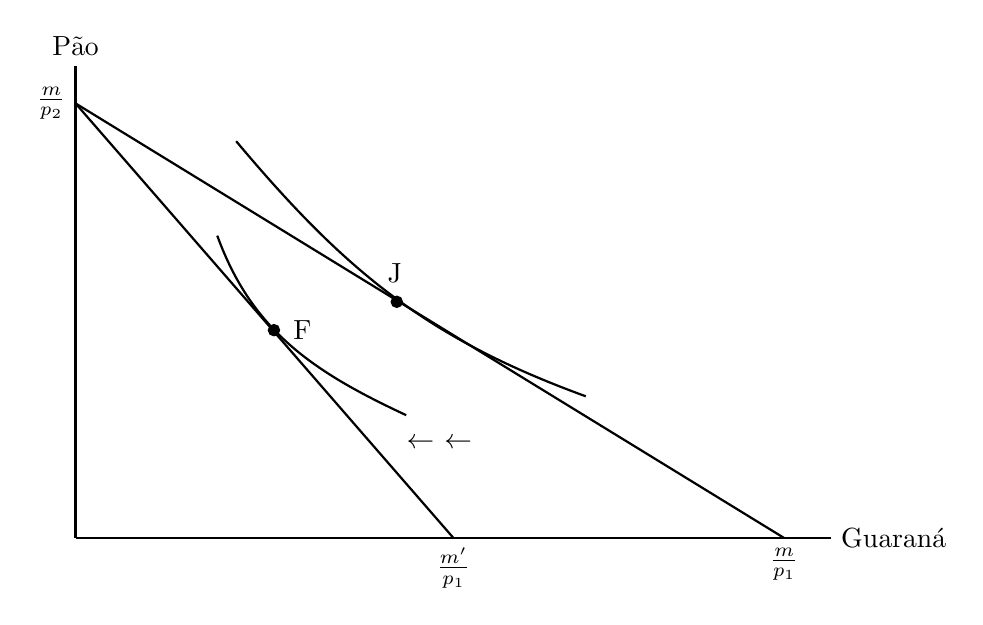
\begin{tikzpicture}[scale=1.2]
	
	\draw [thick] (0,0) -- (8,0);
	
	\draw [thick] (0,0) -- (0,5);
	
	\node [right] at (8,0) {Guaraná};
	\node [below] at (7.5,0) {$\frac{m}{p_{1}}$};
	\node [left] at (0,4.6) {$\frac{m}{p_{2}}$};
	\node [below] at (4,0) {$ \frac{m'}{p_{1}}$};
	\node [above] at (0,5) {Pão};
	
	\draw [thick] (1.7,4.2) to [out=310,in=160] (5.4,1.5);
	
	
	\draw [thick] (1.5,3.2) to [out=290,in=155] (3.5,1.3);
	
	
	\draw [thick] (0,4.6) -- (7.5,0);
	
	\draw [thick] (0,4.6) -- (4,0);
	

	

	

	
	\node [above] at (2.4,2) {F};
	
	\draw[fill] (2.1,2.2) circle [radius =0.06];
	

	\node [right] at (3.2,2.8) {J};
	
	\draw[fill] (3.4,2.5) circle [radius =0.06];
	
	\node [right] at (3.8,1) {$\leftarrow$};

	\node [right] at (3.4,1) {$\leftarrow$};
	
\end{tikzpicture}


\end{center}

As preferências de Renata tiveram uma grande alteração conforme o gráfico acima. Ocasionado pelo aumento de preços.


\singlespacing

\textbf{B)} 


\begin{center}

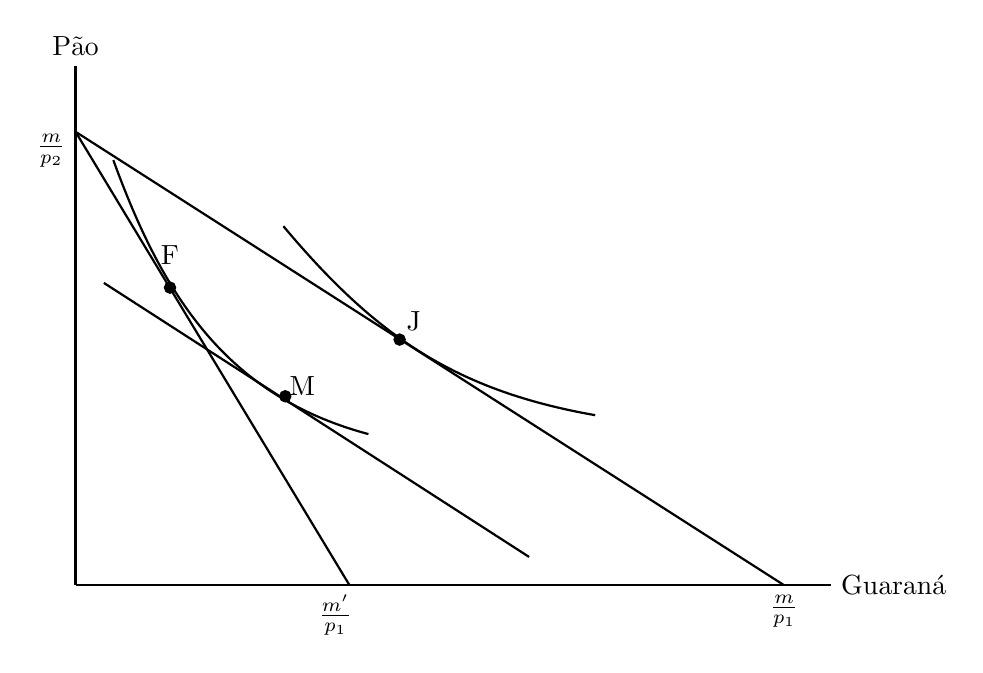
\begin{tikzpicture}[scale=1.2]
	
	\draw [thick] (0,0) -- (8,0);
	
	\draw [thick] (0,0) -- (0,5.5);
	
	\node [right] at (8,0) {Guaraná};
	
	\node [below] at (7.5,0) {$\frac{m}{p_{1}}$};
	\node [left] at (0,4.6) {$\frac{m}{p_{2}}$};
	\node [below] at (2.75,0) {$ \frac{m'}{p_{1}}$};
	
	\node [above] at (0,5.5) {Pão};
	
	\draw [thick] (2.2,3.8) to [out=310,in=170] (5.5,1.8);
	
	\draw [thick] (0.4,4.5) to [out=290,in=165] (3.1,1.6);
	

	

	
	\draw [thick] (0,4.8) -- (7.5,0);
	
	\draw [thick] (0,4.8) -- (2.9,0);
	

	
	\draw [thick] (0.3,3.2) -- (4.8,0.3);
	

	
	\node [above] at (2.4,1.9) {M};
	
	\draw[fill] (2.22,2) circle [radius =0.06];
	

	
	\node [right] at (0.8,3.5) {F};
	
	\draw[fill] (1,3.15) circle [radius =0.06];
	
	\node [right] at (3.4,2.8) {J};
	
	\draw[fill] (3.43,2.6) circle [radius =0.06];
	

	


\end{tikzpicture}
\end{center}

Com a volta do preço do Guaraná ao original, porém com uma redução da renda de Renata em Março (\textbf{M}), ela vai ter a utilidade semelhante a de Fevereiro, por isso \textbf{F} e \textbf{M} estão na mesma curva de indiferença. 

\singlespacing

\textbf{C)} 
\singlespacing
\textbf{C.1)}
\\
Falso. Se ocorresse isso, seria um exemplo de bem de Giffen.
\singlespacing
\textbf{C.2)}
\\
Verdadeiro. Por causa do efeito-substituição que é sempre negativo (no caso de preferências bem-comportadas, negativo).
\singlespacing
\textbf{C.3)}
\\
Falso, só ocorreria se guaraná fosse um bem inferior.
\singlespacing
\textbf{D)}
\\
Nesse caso, não seria verdade. Porque se ocorresse isso, a \textbf{C.1} seria verdadeiro, já que é um caso de bem de Giffen. 
\singlespacing

\textbf{4-}
\singlespacing
\textbf{A)}
\singlespacing

Para encontrar as demandas marshalinas a partir de uma função indireta, iremos usar a identidade de Roy.

\begin{equation}
x_{1}^{m}(\textbf{p},m) = \dfrac{ \partial v(\textbf{p},m) / \partial p_{1}}{\partial v(\textbf{p},m)/\partial m}
$$\\$$
x_{1}^{m}(\textbf{p},m) = - \dfrac{ 50 \left(\dfrac{2}{3}\right)(p_{1}^{\frac{1}{2}}p_{2})^{\frac{-2}{3}-1}m\left(\dfrac{1}{2}\right)p_{1}^{\frac{-1}{2}}p_{2}}{50(p_{1}^{\frac{1}{2}}{p_{2}})^{\frac{-2}{3}}}
$$\\$$
x_{1}^{m}(\textbf{p},m) = \dfrac{m}{3p_{1}}
\end{equation}
Agora, iremos encontrar o $x_{2}$
\begin{equation}
x_{2}^{m}(\textbf{p},m) = \dfrac{ \partial v(\textbf{p},m) / \partial p_{2}}{\partial v(\textbf{p},m)/\partial m}
$$\\$$
x_{2}^{m}(\textbf{p},m) = - \dfrac{50 \left(\dfrac{2}{3} \right) (p_{1}^{\frac{1}{2}}p_{2})^{\frac{-2}{3}-1} mp_{1}^{\frac{1}{2}} }{50(p_{1}^{\frac{1}{2}}p_{2})^{\frac{-2}{3}}}
$$\\$$
x_{2}^{m}(\textbf{p},m) = \dfrac{2m}{3p_{2}}
\end{equation}
Agora, para achar as frações de renda. Utilizaremos as frações de renda.

\begin{equation}
s_{1} = \dfrac{p_{1}x_{1}^{m}(\textbf{p},m)}{m}
$$\\$$
s_{1} = \dfrac{p_{1}\left(\dfrac{m}{3p_{1}}\right)}{m}
$$\\$$
s_{1} = \dfrac{1}{3}
$$\\$$
s_{2} = \dfrac{p_{2}x_{2}^{m}(\textbf{p},m)}{m}
$$\\$$
s_{2} = \dfrac{p_{2}\left(\dfrac{2m}{3p_{2}}\right)}{m}
$$\\$$
$$\\$$
s_{2} = \dfrac{2}{3}
\end{equation}
\singlespacing
\begin{center}
	\section*{Questões José Guilherme - Nota 09}
\end{center}
\singlespacing

\textbf{1-} Considere a função dada por: \\
\begin{center}
	$u(x_{1}x_{2}) = x_{1}^{2}x_{2}$
\end{center}
onde $x_{1}$ e $x_{2}$ são as quantidades consumidas dos bens 1 e 2, respectivamente.

\singlespacing

\textbf{A)} Calcule as funções de demandas Marshallianas e a função de utilidade indireta.
\singlespacing
\textbf{B)} Suponha que os preços dos bens 1 e 2 são $p_{1}$ = R\$ 4 e $p_{2}$ = R\$ 2, respectivamente, e que a renda do consumidor é R\$ 90. Calcule a quantidade consumida de cada bem.
\singlespacing
\textbf{C)} Calcule as elasticidades preço e renda do bem 1. Se a renda aumentar em 10\% você pode dizer o que ocorre com o consumo do bem, sem ter conhecimento do valor original da renda?
\singlespacing
\textbf{D)} Suponha que os preços dos bens e a renda são como dados no item \textbf{B)}. Calcule a variação no excedente do consumidor no caso em que o preço do bem 2 aumenta para R\$ 4.

\singlespacing

\textbf{Respostas:}
\singlespacing

\textbf{A)} 
\\
O primeiro passo é achar as demandas marshallianas.

\begin{equation}
	u(x_{1},x_{2}) = x_{1}^{2}x_{2} \ s.a \ (p_{1}x_{1} + p_{2}x_{2} - m)
$$\\$$
\ell = x_{1}^{2}x_{2} - \lambda(p_{1}x_{1} + p_{2}x_{2} - m)
$$\\$$
\ell = x_{1}^{2}x_{2} -\lambda p_{1}x_{1} - \lambda p_{2}x_{2} + \lambda m $$\\$$
\frac{\partial\ell}{\partial x_{1}} = 2x_{1}x_{2} - \lambda p_{1} = 0
$$\\$$
\frac{\partial\ell}{\partial x_{2}} = x_{1}^{2} - \lambda p_{2} = 0
$$\\$$
\lambda = \lambda
$$\\$$
\dfrac{2x_{1}x_{2}}{p_{1}} = \dfrac{x_{1}^{2}}{p_{2}}
$$\\$$
2x_{1}x_{2}p_{2} = p_{1}x_{1}^{2}
$$\\$$
x_{1} = \dfrac{2x_{2}p_{2}}{p_{1}}
\end{equation}

\begin{center}
Isolando o $x_{1}$
\end{center}

\begin{equation}
\frac{\partial\ell}{\partial \lambda} = -p_{1}x_{1} - p_{2}x_{2} + m = 0
$$\\$$
-p_{1}\left(\dfrac{2x_{2}p_{2}}{p_{1}}\right) - p_{2}x_{2} = -m (-1)
$$\\$$
x_{2}(3p_{2}) = m
$$\\$$
x_{2} = \dfrac{m}{3p_{2}}
\end{equation}

\begin{center}
Substituindo em $x_{1}$
\end{center}

\begin{equation}
x_{1} = \dfrac {2 \left( \dfrac{m}{3p_{2}}\right)p_{2}} {p_{1}}
$$\\$$
x_{1} = \dfrac{2m}{3p_{1}}
$$\\$$
x_{1} = \dfrac{2m}{3p_{1}} \  e \ x_{2} = \dfrac{m}{3p_{2}}
\end{equation}
\begin{center}
Para achar a função indireta, substituiremos as nossas demandas na função original.
\end{center}

\begin{equation}
\vartheta(p_{1},p_{2},m) = x_{1}^{2}x_{2}
$$\\$$
\vartheta(p_{1},p_{2},m) = \left( \dfrac{2m}{3p_{1}} \right)^{2} \left( \dfrac{m}{3p_{2}} \right) =  \dfrac{4}{27} \left(\dfrac{m^{3}}{p_{1}^{2}p_{2}}        \right)
\end{equation}

\singlespacing

\textbf{B)}

\begin{center}
Usando as demandas marshallianas, iremos resolver o problema.
\end{center}

\begin{equation}
p_{1} = 4
$$\\$$
p_{2} = 2
$$\\$$
m = 90
$$\\$$
x_{1} = \dfrac{2 \ x \ 90}{3 \ x \ 4} = 15
$$\\$$
x_{2} = \dfrac{90}{3 \ x \ 2} = 15
\end{equation}

\singlespacing

\textbf{C)} 
\\
\begin{center}
Elasticidade preço:
\end{center}
\begin{equation}
\varepsilon_{1} = \dfrac{p_{1}}{x_{1}} \dfrac{\partial x_{1}}{\partial p_{1}}
$$\\$$
\dfrac{p_{1}}{\frac{2}{3} \frac{m}{p_{1}}} \dfrac{2m}{3p_{1}^{2}} = -1
\end{equation}

\begin{center}
Elasticidade renda:
\end{center}

\begin{equation}
\eta_{1} = \dfrac{m}{x_{1}} \dfrac{\partial x_{1}}{\partial p_{1}}
$$\\$$
\eta_{1} = \dfrac{m}{\frac{2}{3} \frac{m}{p_{1}}} \dfrac{2}{3p_{1}} = 1
\end{equation}
\begin{center}
Por causa da elasticidade unitária, se a renda aumenta em 10\%, consequentemente o consumo do bem 1 aumentará em 10\% também.
\end{center}

\singlespacing

\textbf{D)}
\\
\begin{center}

Para acharmos a variação do excedente do consumidor com as mudanças de preços, iremos fazer os seguintes passos:
\end{center}

\begin{equation}
\Delta EC = \int_{4}^{2} x_{2}(\textbf{p},m) \ dp_{2}
$$\\$$
m = 90
$$\\$$
p_{2} = 2
$$\\$$
p_{2}' = 4
$$\\$$
x_{2} = \dfrac{m}{3p_{2}}
$$\\$$
\Delta EC = -\int_{2}^{4} \dfrac{m}{3p_{2}} \ dp_{2}
$$\\$$
\Delta EC = -\int_{2}^{4} \dfrac{90}{3p_{2}} \ dp_{2}
$$\\$$
\Delta EC = -\int_{2}^{4} \dfrac{1}{3} \left( \dfrac{90}{p_{2}} \right) \ dp_{2}
$$\\$$
\Delta EC = -\int_{2}^{4} 30ln(p_{2})
$$\\$$
\Delta EC = -30[ln(4)-ln(2)]
$$\\$$
\Delta EC = -30.ln(2) = -20,79
\end{equation}

\begin{center}
O aumento de preço gera uma perda de bem-estar ao consumidor. E o valor da perda do seu excedente é de R\$ 20,79.
\end{center}

\singlespacing

\textbf{4-} Considere a mesma função de utilidade do exercício anterior, e suponha que a renda do individuo é R\$ 1.000,00, o preço do bem 1, $p_{1}$ = 1 e o preço do bem 2, $p_{2}$ = 1. Suponha também que o preço do bem 2 aumentou para R\$ 2.
\singlespacing
\textbf{A)} Decomponha o efeito total da mudança de preço do bem 2 em efeito substituição e efeito renda, usando a decomposição de Slutsky (que mantém o poder de compra original constante).
\singlespacing
\textbf{B)} Decomponha o efeito total da mudança de preço do bem 2 em efeito substituição e efeito renda, usando a decomposição de Hicks (que mantém o nível de utilidade original constante).
\singlespacing
\textbf{C)} Calcule o valor de uma compensação de Slutsky. Mostre que essa compensação, que mantém o poder de compra original, aumentará o bem-estar do individuo. Seria possível que a utilidade do individuo fosse menor do que a original com esse tipo de compensação?
Justifique sua resposta.
\singlespacing
\textbf{D)} Calcule o valor de uma compensação de Hicks. Mostre que essa compensação mantém o nível de utilidade constante, e é menor do que a compensação de Slutsky.
\singlespacing
\textbf{E)} Imagine que você é chamado pelo ministro da economia para elaborar uma política de compensação na tarifa de energia elétrica para pessoas com um nível de renda de até R\$ 1.000,00 mensais. Discuta os pontos positivos e negativos de cada uma das compensações vistas acima.

\singlespacing

\textbf{Respostas:}

\singlespacing

\textbf{A)}
\\
Semelhante a questão 3, teremos que ter as funções de demanda marshallianas e os seus dados.
\begin{center}
$m = 1.000$, $p_{1} = 2$, $p_{2} = 1$ e $p_{2}' = 2$
\end{center}
\begin{center}
As demandas marshallianas: $x_{1} = \dfrac{m}{2p_{1}}$ e $x_{2} = \dfrac{m}{2p_{2}}$
\end{center}
Para fazer uma avaliação do efeito total é necessário entender as quantidades dos bens para o $p_{2}$.

\begin{equation}
x_{1} = \dfrac{1.000}{2 \times 1 } = 500
$$\\$$
x_{2} = \dfrac{1000}{2 \times 1} = 500
\end{equation}
Agora mudando os preços do $p_{2}$ de R\$ 1 para R\$ 2.

\begin{equation}
x_{1} = \dfrac{1.000}{2 \times 1} = 500
$$\\$$
x_{2}' = \dfrac{1.000}{2 \times 2} = 250
\end{equation}
\begin{center}
Logo, o efeito total é $ET = x_{2}' - x_{2}$
\\
$ET = 250 - 500$
\\
$ET = -250$ 
\end{center}
Ou seja, nosso efeito total é negativo, já que com o ajuste do preço, sofremos uma perda de 250 quantidades.
\\
Usando a decomposição de Slutsky para calcular o efeito substituição com o poder de compra original.

\begin{equation}
x_{2}^{s}(1,2(500,500)) = \dfrac{1 \times 500 + 2 \times 500}{2 \times 2} = \dfrac{1500}{4} = 375 
\end{equation}

\begin{center}
O ES e EM será:
\end{center}
\begin{equation}
\Delta x_{1} = 375 - 250.
$$\\$$
\Delta x_{1} = 125
$$\\$$
\Delta m = 375 - 250.
$$\\$$ 
\Delta m = 125
\end{equation}

\singlespacing

\textbf{B)}
\\
Usando as demandas hicksianas para essa questão e também a função de utilidade indireta, teremos:

\begin{equation}
$$\\$$
x_{1}^{h}(p_{1},p_{2}, \overline{u}) = p_{1}^{-0,5}p_{2}^{0,5}e^{\frac{\overline{u}}{2}}
$$\\$$
x_{2}^{h}(p_{1},p_{2}, \overline{u}) = p_{1}^{0,5}p_{2}^{-0,5}e^{\frac{\overline{u}}{2}}
\end{equation}

\begin{center}
Usando o $x_{2}$
\end{center}

\begin{equation}
x_{2}^{h}(1,2,ln(500^{2})) = 1^{0,5}2^{-0,5}e^{{\frac{ln(500^{2})}{2}}}
$$\\$$
x_{2}^{h} = \dfrac{500}{\sqrt{2}}
$$\\$$
x_{2}^{h} = 353,55
\end{equation}

\begin{center}
O efeito substituição e renda será:
\end{center}
\begin{equation}
ES = 500 - 353,55
$$\\$$
ES = 146,45
$$\\$$
ER = 353,55 - 250
$$\\$$
ER = 103,55
\end{equation}

\singlespacing

\textbf{C)}
\\
A compensação para os novos preços será de R\$ 500,00. Conforme na parte (68).

\begin{center}
Segue os cálculos abaixo:
\end{center}

\begin{equation}
p_{1} = 1 \ e \ p_{2} = 2
$$\\$$
x_{1}(1,2,1500) = \dfrac{1500}{2 \times 1} = 750
$$\\$$
x_{2}(1,2,1500) = \dfrac{1500}{2 \times 2 } = 375
\end{equation}

\begin{center}
Utilidades anteriores e a atual:
\end{center}

\begin{equation}
u = ln(500^{2}) = ln(250.000)
$$\\$$
u' = ln(750 \times 375) = ln(281.250)
\end{equation}

Então, a utilidade compensada ficou maior que a anterior. Então, é inviável a utilidade do individuo ficar menor do que a compensada, porque com a compensação ele sempre será possível voltar a pelo menos a cesta original.

\singlespacing

\textbf{D)}
\\
 
 \begin{center}
  A variação compensadora de Hicks é:
 \end{center}

\begin{equation}
x_{1} = 500 \ e \ x_{2} = 500.
$$\\$$
u = ln(x_{1}) + ln(x_{2})
$$\\$$
u = ln(500) + ln(500)
$$\\$$
u = 12,43
$$\\$$
(x_{1},x_{2}) = (500,500) = 12,43
$$\\$$
(x_{1}^{*},x_{2}^{*}) = (500,250) =
$$\\$$
ln\left(\dfrac{m}{2}\right) + ln\left(\dfrac{m}{4}\right) = 12,43
$$\\$$
e^{ln(\frac{m}{2}) + ln(\frac{m}{4})} = e12,43 
$$\\$$
e^{ln(\frac{m^{2}}{8})} = e12,43
$$\\$$
\dfrac{m^{2}}{8} = e12,43
$$\\$$
m = (8e12,43)^{1/2}
$$\\$$
m = 1.414,17
\end{equation}

\begin{center}
A VC será de R\$ 414,17. Agora jogaremos saberemos as novas quantidades de utilidades e jogaremos na função original.
\end{center}

\begin{equation}
x_{1} = \dfrac{1.414,17}{2} = 711,32
$$\\$$
x_{2} = \dfrac{1.414,17}{4} = 353,54
$$\\$$
u' = ln(711,32) + ln(353,54) = 12,49
\end{equation}

\singlespacing

\textbf{E)}
\\

\singlespacing

\textbf{7-}  Suponha que a função de utilidade de um consumidor é:

\begin{equation}
u(x_{1},x_{2}) = min \left\{ \dfrac{x_{1}}{\alpha} , \dfrac{x_{2}}{\beta} \right\}
\end{equation}

\textbf{A)} Ilustre graficamente as curvas de indiferença deste consumidor. Determine o caminho da expansão da renda.
\singlespacing
Para os itens d) e e), suponha que $\alpha$ = $\beta$ = 1, a renda do consumidor é R\$ 800,00 e os preços dos dois bens são $p_{1}$ = 2 e $p_{2}$ = 2.
\singlespacing
\textbf{D)} Suponha que o preço do bem 1 aumentou para $\overline{p}_{1}$ = 3. Usando a equação de Slutsky, decomponha esse aumento de preço em efeito substituição e efeito renda. Qual os valores
destes efeitos?

\singlespacing

\textbf{Respostas:}

\singlespacing
\textbf{A)}
\\

\begin{center}
Curva de indiferença:
\end{center}
\begin{equation}
u(x_{1},x_{2}) = min \left\{ \dfrac{x_{1}}{\alpha} , \dfrac{x_{2}}{\beta} \right\}
$$\\$$
x_{2} = \dfrac{\beta}{\alpha} x_{1}
\end{equation}

\begin{center} %Centralização do gráfico a ser desenhado
	\begin{tikzpicture}[scale=0.8] %Início do desenho e definição da escala
	%Eixos
	\draw[->, very thick] (-0.1,0) -- (8.8,0) node[right]{$x_1$}; %Eixo X1
	\draw[->, very thick] (0,-0.1) -- (0,8.8) node[above]{$x_2$}; %Eixo X2
	%Retas
	
	\draw (1.5,2) -- (7,2);
	\draw (1.5,2) -- (1.5,7);
	
	\draw (2.5,3) -- (7,3);
	\draw (2.5,3) -- (2.5,7);
	
	\draw (3.5,4) -- (7,4);
	\draw (3.5,4) -- (3.5,7);
	
	
	\draw[->, very thick, red] (3,2.5) -- (3.5,2.9); 
	\draw[->, very thick, red] (1.7,5.2) -- (2.2,5.5); 
	\draw [thick] (0,0) -- (4,4.9);
	
	
	\draw[->, very thick, red] (4,3.5) -- (4.5,3.9); 
	\draw[->, very thick, red] (2.7,5.2) -- (3.2,5.5);
	
	\draw (0,12) node [right] {Curvas de Indiferença};

		\node [right] at (4,4.9) {$x_{2} = \dfrac{\beta}{\alpha}x_{1}$ $\Rightarrow$ Caminho da expansão da renda};
	\end{tikzpicture}\\
	
	
\end{center} 

\textbf{D)}
\\
Quando os bens $x_{1}$ e $x_{2}$ estão com os preços, $p_{1} = 2$ e $p_{2} = 2$, sabendo da nossa renda m = 800 e $\alpha$ = $\beta$ = 1. Temos os seguintes bens:

\begin{equation}
x_{1} = \dfrac{\alpha m}{\alpha p_{1} + \beta p_{2}}
$$\\$$
x_{2} = \dfrac{\beta m}{\alpha p_{1} + \beta p_{2}}
$$\\$$
x_{1} = \dfrac{1 \times 800}{1 \times 2 + 1 \times 2} = 200
$$\\$$
x_{2} = \dfrac{1 \times 800}{1 \times 2 + 1 \times 2} = 200
\end{equation}

\begin{center}
Agora com o $p_{2}' = 3$
\end{center}

\begin{equation}
x_{1} = \dfrac{1 \times 800}{1 \times 2 + 1 \times 3 } = 160
$$\\$$
x_{2} = \dfrac{1 \times 800}{1 \times 2 + 1 \times 3 } = 160
\end{equation}

\begin{center}
Agora, iremos ver o efeito total dessa mudança.
\end{center}

\begin{equation}
\Delta x_{2} = x_{2}' - x_{2}
$$\\$$
\Delta x_{2} = 160 - 200
$$\\$$
\Delta x_{2} = -40.
\end{equation}

\begin{center}
Agora iremos desenvolver os efeitos usando a equação de Slutsky.
\end{center}

\begin{equation}
$$\\$$
\underbrace{{\dfrac{\partial x_{i}^{M}(\mathbf{p}, m)}{\partial p_{i}}}}_{{\text {efeito total }}}= \underbrace{{\dfrac{\partial x{i}^{h}\left(\mathbf{p}, u^{*}\right)}{\partial p_{i}}}}_{{\text {efeito substituição}}} - \underbrace{ x_{i}^{M}(\mathbf{p}, m) \dfrac{\partial x_{i}^{M}(\mathbf{p}, m)}{\partial m}}_{{\text {efeito renda}}}
$$\\$$
Efeito \ total = \dfrac{\partial x_{1}^{m}}{\partial p_{1}} = - \dfrac{\alpha^{2}m}{(\alpha p_{1} + \beta p_{2})^{2}}
$$\\$$
Efeito \ \text{Substituição} = \dfrac{\partial x_{1}^{h}}{\partial p_{1}}=0
$$\\$$
\text { Efeito Renda: } \quad-x_{1}^{M} \frac{\partial x_{1}^{M}}{\partial m}=-\frac{\alpha^{2} m}{\left(\alpha p_{1}+\beta p_{2}\right)^{2}}
\end{equation}

\singlespacing

\begin{center}
	\section*{Questões José Guilherme - Nota 10}
\end{center}

\singlespacing

\textbf{1-} Suponha que existam apenas 3 bens e que um certo individuo escolhe as cestas $\textbf{x}^{i}$ = ($x_{1}^{i},x_{2}^{i},x_{3}^{i}$) aos preços $\textbf{p}^{i}$ = ($p_{1}^{i},p_{2}^{i},p_{3}^{i}$), i = 1,2,3 (logo, existem três observações de consumo desse
individuo), onde:

\begin{equation}
\text{Observação 1:} \ \  \textbf{p}^{1} = (1,1,2), \ \textbf{x}^{1} = (5,19,9)
$$\\$$
\text{Observação 2:} \ \  \textbf{p}^{2} = (1,1,1), \ \textbf{x}^{2} = (12,12,12)
$$\\$$
\text{Observação 3:} \ \  \textbf{p}^{3} = (1,2,1), \ \textbf{x}^{3} = (27,11,1)
\end{equation}
\singlespacing
\textbf{A)} Mostre que essas observações satisfazem o Axioma Fraco da preferência revelada.

\singlespacing

\textbf{Respostas:}

\textbf{A)} 
\begin{center}

$\begin{array}{|l|c|c|c|}
	\hline & \text { Cesta Obs 1 } & \text { Cesta Obs 2 } & \text { Cesta Obs 3 } \\
	\hline \text { Preços Obs 1 } & 42 & 48 & 40(*) \\
	\hline \text { Preços Obs 2 } & 33\left(^{*}\right) & 36 & 39 \\
	\hline \text { Precos Obs 3 } & 52 & 48\left(^{*}\right) & 50 \\
	\hline
\end{array}$
\end{center}
\singlespacing
O \textbf{AFrPR} (Axioma fraco da preferência revelada) é caracterizado por não ter transitividade. Já que o axioma define que a cesta \textbf{x} é sempre preferida a cesta \textbf{y} e que não pode ocorrer o inverso.

Sabendo desses detalhes, temos que:

\begin{equation}
\begin{aligned}
&\mathrm{x}{1} \succeq{R}^{D} \mathrm{x}{3} \text { mas não ocorre } \mathrm{x}{3} \succeq_{R}^{D} \mathrm{x}_{1}\\
&\mathrm{x}{2} \succeq{R^{D}} \mathrm{x}{1} \text { mas não ocorre } \mathrm{x}{1} \succeq_{R^{D}} \mathrm{x}_{2}\\
\end{aligned}
\end{equation}

\singlespacing

\begin{center}
	\section*{Questões José Guilherme - Nota 11}
\end{center}

\singlespacing

\textbf{1-} Um consumidor tem uma função utilidade \textit{u}($x_{1}, x_{2}$) = $x_{1}^{0,5}x_{2}^{0,5}$ e uma dotação inicial de $\textit{e}_{1}$ = 2 e $\textit{e}_{2}$ = 1.

\singlespacing

\textbf{A)} Resolva o problema do consumidor e encontre as demandas brutas pelos bens.

\singlespacing

\textbf{B)} Suponha que os preços dos dois bens sejam $p_{1}$ = $p_{2}$ = 1. Calcule a demanda ótima nesse caso. O consumidor é vendedor liquido de algum dos bens?

\singlespacing

\textbf{C)} Suponha que o preço do bem 1 diminui de 1 para $\overline{p}_{1}$ = 0,9. O que ocorre nesse caso com o bem-estar do consumidor?

\singlespacing

\textbf{D)} Suponha agora que o preço do bem 1 diminui de 1 para $\overline{p}_{1}$ = 0,1. O que ocorre nesse caso com o bem-estar do consumidor? Compare com o item anterior.

\singlespacing

\textbf{Respostas:}

\singlespacing

\textbf{A)}

\begin{equation}
u(x_{1},x_{2}) = x_{1}^{0,5}x_{2}^{0,5} \ s.a \ (p_{1}x_{1} + p_{2}x_{2} = p_{1}\textit{e}_{1} + p_{2}\textit{e}_{2})
$$\\$$
\ell = x_{1}^{0,5}x_{2}^{0,5} + \lambda(-p_{1}x_{1} - p_{2}x_{2} + p_{1}\textit{e}_{1} + p_{2}\textit{e}_{2})
$$\\$$
\ell = x_{1}^{0,5}x_{2}^{0,5} -\lambda p_{1}x_{1} - \lambda p_{2}x_{2} + \lambda p_{1}\textit{e}_{1} + \lambda p_{2}\textit{e}_{2} 
$$\\$$
\frac{\partial\ell}{\partial x_{1}} = 0,5x_{1}^{-0,5}x_{2}^{0,5} - \lambda p_{1} = 0
$$\\$$
\frac{\partial\ell}{\partial x_{2}} = x_{1}^{0,5}x_{2}^{-0,5} - \lambda p_{2} = 0
$$\\$$
\lambda = \lambda
$$\\$$
\dfrac{0,5x_{1}^{-0,5}x_{2}^{0,5}}{p_{1}} = \dfrac{0,5x_{1}^{0,5}x_{2}^{-0,5}}{p_{2}}
$$\\$$
x_{2}p_{2} = x_{1}p_{1}
$$\\$$
x_{2} = \dfrac{x_{1}p_{1}}{p_{2}}
\end{equation}

\begin{center}
Agora isolando $x_{2}$ e substituindo na função.
\end{center}

\begin{equation}
\frac{\partial\ell}{\partial \lambda} = -p_{1}x_{1} - p_{2}x_{2} + p_{1}\textit{e}_{1} + p_{2}\textit{e}_{2} = 0
$$\\$$
-p_{1}x_{1} - p_{2}\left(\dfrac{x_{1}p_{1}}{p_{2}}\right) = -p_{1}\textit{e}_{1} - p_{2}\textit{e}_{2}
$$\\$$
-2p_{1}x_{1} = -p_{1}\textit{e}_{1} - p_{2}\textit{e}_{2} (-1)
$$\\$$
x_{1} = \dfrac{p_{1}\textit{e}_{1} + p_{2}\textit{e}_{2}}{2p_{1}}
\end{equation}

\begin{center}
Substituindo $x_{1}$ em $x_{2}$
\end{center}

\begin{equation}
x_{2} = \dfrac{\left( \dfrac{p_{1}\textit{e}_{1} + p_{2}\textit{e}_{2}}{2p_{1}}\right)\cdot p_{1}}{p_{2}}
$$\\$$
x_{2} = \dfrac{p_{1}\textit{e}_{1} + p_{2}\textit{e}_{2}}{2p_{2}}
\end{equation}

\begin{center}
As demandas brutas $x_{1}$ e $x_{2}$ serão as seguintes:

\begin{equation}
x_{1} = \dfrac{p_{1}\textit{e}_{1} + p_{2}\textit{e}_{2}}{2p_{1}}
$$\\$$
x_{2} = \dfrac{p_{1}\textit{e}_{1} + p_{2}\textit{e}_{2}}{2p_{2}}
\end{equation}

\end{center}

\singlespacing

\textbf{B)} Sabendo que $p_{1} = p_{2} = 1$ ; $\textit{e}_{1} = 2$  $\textit{e}_{2} = 1$, então, sabemos que $p_{1}\textit{e}_{1} + p_{2}\textit{e}_{2} = 3$.

\begin{equation}
x_{1}(1,1,3) = \dfrac{3}{2} = 1,5.
$$\\$$
x_{2}(1,1,3) = \dfrac{3}{2} = 1,5.
\end{equation}

\begin{center}
Dá para compreender que o individuo é vendedor do bem $x_{1}$ e consumidor do bem $x_{2}$.
\end{center}

\singlespacing

\textbf{C)} Sabendo que $p_{1} = p_{2} = 1$ ; $\textit{e}_{1} = 2$  $\textit{e}_{2} = 1$, então, sabemos que $p_{1}\textit{e}_{1} + p_{2}\textit{e}_{2} = 3$. Porém, sabemos que o $p_{1}$ haverá uma queda, da seguinte forma $\overline{p}_{1}$ = 0,9. Também, $p_{1}\textit{e}_{1} + p_{2}\textit{e}_{2} = 2,8$.

\begin{equation}
x_{1}(0,9;1;2,8) = \dfrac{2,8}{2 \cdot 0,9} = 1,55
$$\\$$
x_{2}(0,9;1;2,8) = \dfrac{2,8}{2 \cdot 1} = 1,4
\end{equation}

\begin{center}
Agora iremos entender o impacto de bem-estar com a mudança de preços.
\end{center}

\begin{equation}
p_{1} = 1 \ ; \ \textit{u}(x_{1}, x_{2}) = (1,5)^{0,5} \cdot (1,5)^{0,5} = 1,5. 
$$\\$$
\overline{p_{1}} = 0,9 \ ; \ \textit{u}(x_{1}, x_{2}) = (1,55)^{0,5} \cdot (1,4)^{0,5} = 1,473.
\end{equation}

\begin{center}
Ou seja, ocorre uma queda de bem-estar decorrentes do preços.
\end{center}

\singlespacing

\textbf{D)}  Sabendo que $p_{1} = p_{2} = 1$ ; $\textit{e}_{1} = 2$  $\textit{e}_{2} = 1$, então, sabemos que $p_{1}\textit{e}_{1} + p_{2}\textit{e}_{2} = 3$. Porém, sabemos que o $p_{1}$ haverá uma queda, da seguinte forma $\overline{p}_{1}$ = 0,1. Também, $p_{1}\textit{e}_{1} + p_{2}\textit{e}_{2} = 1,2$.

\begin{equation}
x_{1}(0,1;1;1,2) = \dfrac{1,2}{2 \cdot 0,1} = 6
$$\\$$
x_{2}(0,1;1;1,2) = \dfrac{1,2}{2 \cdot 1} = 0,6
\end{equation}

\begin{equation}
p_{1} = 1 \ ; \ \textit{u}(x_{1}, x_{2}) = (1,5)^{0,5} \cdot (1,5)^{0,5} = 1,5. 
$$\\$$
\overline{p_{1}} = 0,1 \ ; \ \textit{u}(x_{1}, x_{2}) = (6)^{0,5} \cdot (0,6)^{0,5} = 1,90.
\end{equation}

\begin{center}
O nível de preço de 0,1 gera uma utilidade tão grande, que o individuo passa de vendedor para consumidor no bem $x_{1}$.
\end{center}


\singlespacing


\textbf{4-} Um consumidor tem uma função utilidade \textit{u}($x_{1}, x_{2}$) = $x_{1}x_{2}$ e uma dotação inicial de $\textit{e}_{1}$ = 1 e $\textit{e}_{2}$ = 5.

\singlespacing

\textbf{A)} Resolva o problema do consumidor e encontre as demandas brutas pelos bens.

\singlespacing

\textbf{B)} Suponha que os preços dos dois bens sejam $p_{1} = p_{2} $ = 1. Calcule a demanda ótima nesse caso. O consumidor é vendedor liquido de algum dos bens?

\singlespacing

\textbf{C)} Suponha que o preço do bem 1 diminui de 1 para $\overline{p}_{1}$ = 0,5. O que ocorre nesse caso com a demanda ótima dos bens 1 e 2 e com o bem-estar do consumidor?

\singlespacing

\textbf{D)} Calcule os efeitos substituição, renda tradicional e renda dotação para a mudança de preço descrita no item anterior. Como se comportam os sinais dos efeitos renda tradicional e renda dotação?

\singlespacing

\textbf{Respostas:}

\singlespacing

\textbf{A)}

\begin{equation}
u(x_{1},x_{2}) = x_{1}x_{2} \ s.a \ (p_{1}x_{1} + p_{2}x_{2} = p_{1}\textit{e}_{1} + p_{2}\textit{e}_{2})
$$\\$$
\ell = x_{1}x_{2} + \lambda(-p_{1}x_{1} - p_{2}x_{2} + p_{1}\textit{e}_{1} + p_{2}\textit{e}_{2})
$$\\$$
\ell = x_{1}x_{2} -\lambda p_{1}x_{1} - \lambda p_{2}x_{2} + \lambda p_{1}\textit{e}_{1} + \lambda p_{2}\textit{e}_{2} 
$$\\$$
\frac{\partial\ell}{\partial x_{1}} = x_{2} - \lambda p_{1} = 0
$$\\$$
\frac{\partial\ell}{\partial x_{2}} = x_{1} - \lambda p_{2} = 0
$$\\$$
\lambda = \lambda
$$\\$$
\dfrac{x_{2}}{p_{1}} = \dfrac{x_{1}}{p_{2}}
$$\\$$
x_{2}p_{2} = x_{1}p_{1}
$$\\$$
x_{2} = \dfrac{x_{1}p_{1}}{p_{2}}
\end{equation}

\begin{center}
	Agora isolando $x_{2}$ e substituindo na função.
\end{center}

\begin{equation}
\frac{\partial\ell}{\partial \lambda} = -p_{1}x_{1} - p_{2}x_{2} + p_{1}\textit{e}_{1} + p_{2}\textit{e}_{2} = 0
$$\\$$
-p_{1}x_{1} - p_{2}\left(\dfrac{x_{1}p_{1}}{p_{2}}\right) = -p_{1}\textit{e}_{1} - p_{2}\textit{e}_{2}
$$\\$$
-2p_{1}x_{1} = -p_{1}\textit{e}_{1} - p_{2}\textit{e}_{2} (-1)
$$\\$$
x_{1} = \dfrac{p_{1}\textit{e}_{1} + p_{2}\textit{e}_{2}}{2p_{1}}
\end{equation}

\begin{center}
	Substituindo $x_{1}$ em $x_{2}$
\end{center}

\begin{equation}
x_{2} = \dfrac{\left( \dfrac{p_{1}\textit{e}_{1} + p_{2}\textit{e}_{2}}{2p_{1}}\right)\cdot p_{1}}{p_{2}}
$$\\$$
x_{2} = \dfrac{p_{1}\textit{e}_{1} + p_{2}\textit{e}_{2}}{2p_{2}}
\end{equation}

\begin{center}
	As demandas brutas $x_{1}$ e $x_{2}$ serão as seguintes:
\end{center}

\begin{equation}
x_{1} = \dfrac{p_{1}\textit{e}_{1} + p_{2}\textit{e}_{2}}{2p_{1}}
$$\\$$
x_{2} = \dfrac{p_{1}\textit{e}_{1} + p_{2}\textit{e}_{2}}{2p_{2}}
\end{equation}

\singlespacing

\textbf{B)}

Sabendo que $p_{1} = p_{2} = 1$ ; $\textit{e}_{1} = 2$  $\textit{e}_{2} = 5$, então, sabemos que $p_{1}\textit{e}_{1} + p_{2}\textit{e}_{2} = 6$.

\begin{equation}
x_{1}(1,1,6) = \dfrac{6}{2} = 3.
$$\\$$
x_{2}(1,1,6) = \dfrac{6}{2} = 3.
\end{equation}

\begin{center}
	Dá para compreender que o individuo é vendedor do bem $x_{1}$ e consumidor do bem $x_{2}$.
\end{center}

\singlespacing

\textbf{C)}

Sabendo que $p_{1} = p_{2} = 1$ ; $\textit{e}_{1} = 2$  $\textit{e}_{2} = 1$, então, sabemos que $p_{1}\textit{e}_{1} + p_{2}\textit{e}_{2} = 6$. Porém, sabemos que o $p_{1}$ haverá uma queda, da seguinte forma $\overline{p}_{1}$ = 0,5. Também, $p_{1}\textit{e}_{1} + p_{2}\textit{e}_{2} = 5,5$.

\begin{equation}
x_{1}(0,5;1;5,5) = \dfrac{5,5}{2 \cdot 0,5} = 5,5
$$\\$$
x_{2}(0,5;1;5,5) = \dfrac{5,5}{2 \cdot 1} = 2,75
\end{equation}

\begin{center}
	Agora iremos entender o impacto de bem-estar com a mudança de preços.
\end{center}

\begin{equation}
p_{1} = 1 \ ; \ \textit{u}(x_{1}, x_{2}) = (3) \cdot (3) = 9. 
$$\\$$
\overline{p_{1}} = 0,5 \ ; \ \textit{u}(x_{1}, x_{2}) = (5,5) \cdot (2,75) = 15,125.
\end{equation}

\begin{center}
	Ou seja, ocorre um movimento inverso que a utilidade aumentou conforme a diminuição do preço.
\end{center}

\begin{center}
	\section*{Questões José Guilherme - Nota 12}
\end{center}

\singlespacing

\textbf{1- } Suponha que Paulo tem R\$ 1000 hoje e espera receber R\$1000 em um ano. Paulo não tem outra renda, e ele pode poupar ou pegar emprestado a uma taxa de juros de 25\% ao ano.

\singlespacing

\textbf{A)} Qual o máximo que Paulo pode gastar no ano que vem? Qual o máximo que Paulo pode gastar hoje?

\singlespacing

\textbf{B)} Suponha que Paulo toma emprestado R\$ 800 e consome R\$ 1800 hoje. Quanto ele terá para consumir no ano que vem?

\singlespacing

\textbf{C)} Desenhe a reta orçamentária de Paulo, entre “consumo hoje” (eixo x) e “consumo ano que vem” (eixo y). Qual é a inclinação dessa reta? Qual a interpretação econômica dessa inclinação?

\singlespacing

\textbf{D)} Mostre como a reta orçamentária se desloca para os dois casos abaixos:

\singlespacing

\textbf{i)} Paulo acha R\$ 400 em uma gaveta hoje.
\\
\textbf{ii)} Paulo descobre que vai receber no ano que vem R\$ 500 de uma herança.

\singlespacing

\textbf{E)} Volte a supor que Paulo tem R\$ 1000 hoje e terá R\$ 1000 no ano que vem. Paulo escolhe não poupar nem tomar emprestado. Ilustre a tangência do curva de indiferença de Paulo com a sua reta orçamentária. 

\singlespacing

\textbf{F)} Suponha que Paulo usa o seu dinheiro conforme o item e), quando a taxa de juros for 25\%. Porém a taxa de juros aumentou hoje para 50\%. Paulo altera o seu consumo hoje? Ele está melhor ou pior do que antes?

\singlespacing

\textbf{G)} Decomponha a mudança no consumo de Paulo ocorrida no item f) em efeito substituição e efeito renda. Determine, se possível, as direções do efeito substituição e do efeito renda.

\singlespacing

\textbf{4-} (NS) Laibson (1997) supõe que as pessoas possuem uma utilidade intertemporal com a seguinte forma:

\begin{equation}
U\left(c_{t}, c_{t+1}, \ldots, c_{T}\right)=u\left(c_{t}\right)+\beta \sum_{k=1}^{T-t} \delta^{k} u\left(c_{t+k}\right)
\end{equation}

Com T $>$ t, 0 $<$ $\beta$ $<$ 1 e 0 $<$ $\delta$ $<$ 1. Este tipo particular de desconto intertemporal leva a
possibilidade de miopia.

\singlespacing

\textbf{A)} Laibson sugere que $\beta$ = 0,66 e $\delta$ = 0,99. Mostre que para esses valores, os fatores pelos
quais consumo futuro é descontado seguem um padrão hiperbólico (isto é, que esses
fatores caem abruptamente em t + 1 e depois seguem uma taxa de declínio geométrico
ao longo do tempo).

\singlespacing

\textbf{D)} Descreva alguns modos que as pessoas procuram restringir as suas escolhas futuras no
mundo real.

\singlespacing

\textbf{Respostas:}

\singlespacing

\textbf{1-}

\singlespacing

\textbf{A)}
\\
Paulo tem hoje = R\$ 1.000 e sabendo que a taxa de juros é 25\% a.a, usando as nossas restrições, podemos aplicar da seguinte forma:

\begin{equation}
c_{2} = m_{1}(1+r) + m_{2}
$$\\$$
c_{2} = 1.000(1+0,25) + 1.000
$$\\$$
c_{2} = 2.250
\end{equation}

Ou seja, R\$ 2.250,00 será o máximo que Paulo poderá gastar no ano que vem.
\\
Agora, no presente, usaremos a seguinte restrição:

\begin{equation}
c_{1} = m_{1} + \left(\dfrac{1}{1 + r}\right) \cdot m_{2}
$$\\$$
c_{1} = 1.000 + \left( \dfrac{1}{1 + 0,25} \right) \cdot 1.000
$$\\$$
c_{1} = 1.800
\end{equation}

Paulo poderá gastar apenas R\$ 1.800,00 no presente.

\singlespacing

\textbf{B)} 
\\
Não tera nada a consumir, vejamos, se Paulo gasta os R\$ 1.800,00 e pega R\$ 800,00 emprestados a uma taxa de 25\% a.a, ele terá que pagar R\$ 1.000,00 no ano posterior.

\singlespacing

\textbf{C)} 
\\
O primeiro passo é entender como funciona o gráfico: 

\begin{center}
	\begin{tikzpicture}[scale=1] 
	
	\draw[->, very thick] (-0.1,0) -- (8,0) node[right]{$c_1$}; 
	\draw[->, very thick] (0,-0.1) -- (0,8) node[above]{$c_2$};
	\draw (0,7) -- (7,0) node[below]{$m_{1} + \left( \dfrac{1}{1 + r} \right) \cdot m_{2}$}; 
	\node[left] at (0,7){$(1 + r)m_{1} + m_{2}$};
	\draw[dashed] (3,4) -- (3,0);
	\draw[dashed] (3,4) -- (0,4);
	\node[below] at (3,0){$m_{1}$};
	\node[left] at (0,4){$m_{2}$};
	\draw (3.1,4.1) node [right]  {$\text{Inclinação} -(1+r)$};
	\end{tikzpicture}
\end{center}

Ou seja, dessa maneira podemos plotar os nossos dados, ficando da seguinte maneira:

\begin{equation}
c_{1} = 1.000 + \left(\dfrac{1}{1 + 0,25} \right) \cdot 1.000
$$\\$$
c_{1} = 1.800
$$\\$$
c_{2} = (1 + 0,25) \cdot 1.000 + 1.000
$$\\$$
c_{2} = 2.250
\end{equation}

\begin{center}
	\begin{tikzpicture}[scale=1] 
	
	\draw[->, very thick] (-0.1,0) -- (8,0) node[right]{$c_1$}; 
	\draw[->, very thick] (0,-0.1) -- (0,8) node[above]{$c_2$};
	\draw (0,7) -- (7,0) node[below]{$1.800$}; 
	\node[left] at (0,7){$2.250$};
	\draw[dashed] (3,4) -- (3,0);
	\draw[dashed] (3,4) -- (0,4);
	\node[below] at (3,0){$1.000$};
	\node[left] at (0,4){$1.000$};
	\draw (3.1,4.1) node [right]  {$-1,25$};
	\end{tikzpicture}
\end{center}

Ou seja, a interpretação econômica é que essa inclinação é uma relação do consumo hoje com o consumo futuro, essa inclinação nos informa como é a relação deste agente com a decisão de consumir no período que deseja. 

\singlespacing

\textbf{D)} 
\\
\textbf{i)} Se o Paulo pegue essa nova quantia, teremos os seguintes dados.

\begin{equation}
c_{1} = 1.400 + \left( \dfrac{1}{1 + 0,25} \right) \cdot 1.000
$$\\$$
c_{1} = 2.120
\end{equation}

\begin{center}
	\begin{tikzpicture}[scale=1] 
	
	\draw[->, very thick] (-0.1,0) -- (10,0) node[right]{$c_1$}; 
	\draw[->, very thick] (0,-0.1) -- (0,10) node[above]{$c_2$};
	\draw (0,7) -- (7,0) node[below]{$1.800$}; 
	\draw (0,7) -- (8.6,0) node[below]{$2.120$}; 
	\node[left] at (0,7){$2.250$};
	\end{tikzpicture}
\end{center}

\singlespacing

\textbf{ii)}
\\
Se Paulo descobrir uma herança no valor de R\$ 500,00 no próximo ano. Teremos as seguintes alterações: 

\begin{equation}
c_{2} = (1 + 0,25) \cdot 1.500 + 1.000
c_{2} = 2.875
\end{equation}

\begin{center}
	\begin{tikzpicture}[scale=1] 
	
	\draw[->, very thick] (-0.1,0) -- (10,0) node[right]{$c_1$}; 
	\draw[->, very thick] (0,-0.1) -- (0,10) node[above]{$c_2$};
	\draw (0,7) -- (7,0) node[below]{$1.800$}; 
	\draw (0,8) -- (7,0);
	\node[left] at (0,7){$2.250$};
	\node[left] at (0,8){$2.875$};
	\end{tikzpicture}
\end{center}

\singlespacing

\textbf{E)} 
\\
Se Paulo tiver R\$ 1.000 hoje e R\$ 1.000 no ano que vem, a reta orçamentária será: 

\begin{center}


	
	\begin{tikzpicture}[scale=.9]
	
	\draw (0,7.7) node [left] {$c_{2}$} -- (0,0) node [below left] {$ $} -- (8.2,0) node [below right] {$c_{1}$};
	
	\node [left] at (0,6.1) {$2.250$};
	
	\node [below] at (5.75,0) {$1.800$};
	
	\node [below] at (2.9,0) {$1.000$};
	
	\node [left] at (0,3) {$1.000$};
	
	\node [right] at (6,1.4) {$ $};
	
	
	\draw [dotted, thick] (0,3) -- (2.9,3) -- (2.9,0);
	
	\draw (1.5,6.4) to [out=-90, in=130] (2.9,3) to [out=-50, in=170] (6,1.4);
	
	\draw (0,6.1) -- (5.75,0);
	
	\end{tikzpicture}
	

	
\end{center}

Assim, será a curva de indiferença do Paulo.

\singlespacing

\textbf{F)} 
\\
Sabendo que a taxa de juros irá subir para 50\% a.a, agora podemos fazer os novos cálculos:
\\
Paulo terá a mesma renda, porém agora só irá alterar a taxa de juros.

\begin{equation}
c_{1} = 1.000 + \left( \dfrac{1}{1 + 0,50} \right) \cdot 1.000
$$\\$$
c_{1} = 1.666,67
$$\\$$
c_{2} = (1 + 0,50) \cdot 1.000 + 1.000
$$\\$$
c_{2} = 2.500
\end{equation}

Ou seja, Paulo irá consumir R\$ 1.666,67 hoje e R\$ 2.500,00 no futuro.

\singlespacing

\textbf{G)} 
\\
\begin{center}
	
	
	
	\begin{tikzpicture}[scale=.9]
	
	\draw (0,7.7) node [left] {$c_{2}$} -- (0,0) node [below left] {$ $} -- (8.2,0) node [below right] {$c_{1}$};
	
	\node [left] at (0,6.1) {$2.250$};
	
	\node [below] at (6.3,0) {$1.800$};
	
	\node [below] at (2.9,0) {$1.000$};
	
	\node [left] at (0,3) {$1.000$};
	
	\node [right] at (6,1.4) {$ $};
	
	
	\draw [dotted, thick] (0,3) -- (2.9,3) -- (2.9,0);
	
	\draw (1.3,5.9) to [out=280,in=190] (5.1,2.5);
	
	\draw (0,6.1) -- (6,0);
	
	\draw (0,7) -- (4.9,0);
	\node [left] at (0,7) {$2.500$};
	\node [below] at (4.9,0) {$1.666$};
	
	\end{tikzpicture}
	
\end{center}

Assim, sabendo que o ES é sempre negativo, sabemos que quando aumenta a taxa de juros, o Paulo deixa de consumir hoje para consumir no próximo ano e o ER será negativo também, já que com o aumento da taxa de juros, ele vai deixar de consumir hoje.

\singlespacing

\textbf{4-}
\singlespacing

\textbf{A)} 
\\
O grande problema dessa questão está no t + 1, quando temos o valor do presente (t) é demonstrado que não há um desconto, ou seja, num primeiro período vai ocorrer uma queda brusca, apenas os valores futuros de (t + 1) irão ter um desconto de $\beta$ = 0,66. Ou seja, a utilidade de se consumir num futuro a seguir é premiada pelos descontos de  $\delta$ = 0,99 e $\beta$ = 0,66.

\singlespacing

\textbf{D)} 
\\
Fundos de pensão, aposentadorias como o sistema brasileiro, sistemas de poupança. 

\singlespacing

\begin{center}
\section*{Questões José Guilherme - Nota 13}
\end{center}

\textbf{1-} Considere as loterias $g=(0,50 \circ 100 ; 0,50 \circ 1000)$ e $h=(0,20 \circ 100 ; 0,30 \circ 25 ; 0,50 \circ 16)$. Calcule a utilidade esperada, o equivalente de certeza, o prêmio de risco dessas duas loterias para casos abaixo:
\\
a) $u(w)=\sqrt{w}, w_{0}=100$
\\
b) $u(w)=\sqrt{w}, w_{0}=50$.
\\
c) $u(w)=w, w_{0}=100$.
\\
d) $u(w)=w, w_{0}=50$.
\\
e) $u(w)=w^{2}, w_{0}=100$.
\\
f) $u(w)=w^{2}, w_{0}=50$.

\singlespacing

\textbf{Resposta:}

\textbf{A)}

A nossa utilidade esperada é calculada da seguinte forma:

\begin{equation}
	U(w) = \sqrt{w} ,   w_{0} = 100
\end{equation}

\begin{enumerate}
	\item Utilidade esperada
	\begin{equation}
		U(g) = 0,5 \cdot \sqrt{100 + 100} + 0,5 \cdot \sqrt{100 + 1000}
		$$\\$$
		U(g) = 0,5 \cdot 10\sqrt{2}  + 0,5 \cdot 10 \sqrt{11}
		$$\\$$
		U(g) = 5 \sqrt{2} + 5\sqrt{11}
		$$\\$$
		U(g) = 23,65
	\end{equation}
	
	\begin{equation}
		U(h) = 0,2 \cdot \sqrt{100 + 100} + 0,3 \cdot \sqrt{100 + 25} + 0,5 \cdot \sqrt{100 +16}
		$$\\$$
		U(h) = 0,2 \cdot 10\sqrt{2}  + 0,3 \cdot 5 \sqrt{5} + \sqrt{29}
		$$\\$$
		U(h) = 2 \sqrt{2} + 1,5\sqrt{5} + \sqrt{29}
		$$\\$$
		U(h) = 11,57
	\end{equation}
	\\ Essas são as utilidades esperadas de $g$ e $h$
	
	\item Equivalente de certeza
	
	\begin{equation}
	\sqrt{100 + EC_{g}} = U(g)
	$$\\$$
	\sqrt{100 + EC_[g]} = 23,65
	$$\\$$
	EC_{g} = 23,65^{2} - 100
	$$\\$$
	EC_{g} = 559,32 - 100
	$$\\$$
	EC_{g} = 459,32
	\end{equation}
	
	\begin{equation}
	\sqrt{100 + EC_{h}} = U(h)
	$$\\$$
	\sqrt{100 + EC_[h]} = 11,57
	$$\\$$
	EC_{h} = 11,57^{2} - 100
	$$\\$$
	EC_{h} = 133,86 - 100
	$$\\$$
	EC_{h} = 33,86
	\end{equation}
	\\ Essas são as nossas equivalências de certeza $g$ e $h$.
	
	\item Valor esperado
	
	\begin{equation}
		Eg = 0,5 \cdot 100 + 0,5 \cdot 1.000 = 550
		$$\\$$
		Eh = 0,2 \cdot 100 + 0,3 \cdot 25 + 0,5 \cdot 16 = 35,50
	\end{equation}
	Estes são os nossos valores esperados de $g$ e $h$.
	
	\item Prêmio de risco
	
	\begin{equation}
	Pg = E(g) - EC(g)
	$$\\$$
	Pg = 550 - 451,32
	$$\\$$
	Pg = 90,68
	\end{equation}
	
	\begin{equation}
		Ph = E(h) - EC(h)
		$$\\$$
		Ph = 35,50 - 33,86
		$$\\$$
		Ph = 1,64 
	\end{equation}
	
	Nesse caso, como os prêmios de riscos estão maiores que 0, logo, o individuo nesse caso é averso a risco.
\end{enumerate}

\singlespacing

\textbf{B)}

A nossa utilidade esperada é calculada da seguinte forma:

\begin{equation}
U(w) = \sqrt{w} ,   w_{0} = 50
\end{equation}

\begin{enumerate}
	\item Utilidade esperada
	\begin{equation}
	U(g) = 0,5 \cdot \sqrt{50 + 100} + 0,5 \cdot \sqrt{50 + 1000}
	$$\\$$
	U(g) = 0,5 \cdot 5\sqrt{6}  + 0,5 \cdot 5 \sqrt{42}
	$$\\$$
	U(g) = 2,5 \sqrt{6} + 2,5\sqrt{42}
	$$\\$$
	U(g) = 22,32
	\end{equation}
	
	\begin{equation}
	U(h) = 0,2 \cdot \sqrt{50 + 100} + 0,3 \cdot \sqrt{50 + 25} + 0,5 \cdot \sqrt{50 + 16}
	$$\\$$
	U(h) = 0,2 \cdot 5\sqrt{6}  + 0,3 \cdot 5 \sqrt{3} + 0,5\sqrt{66}
	$$\\$$
	U(h) =  \sqrt{6} + 1,5\sqrt{3} + 0,5 \sqrt{29}
	$$\\$$
	U(h) = 9,11
	\end{equation}
	\\ Essas são as utilidades esperadas de $g$ e $h$
	
	\item Equivalente de certeza
	
	\begin{equation}
	\sqrt{50 + EC_{g}} = U(g)
	$$\\$$
	\sqrt{50 + EC_[g]} = 22,32
	$$\\$$
	EC_{g} = 22,32^{2} - 50
	$$\\$$
	EC_{g} = 498,18 - 50
	$$\\$$
	EC_{g} = 448,18
	\end{equation}
	
	\begin{equation}
	\sqrt{50 + EC_{h}} = U(h)
	$$\\$$
	\sqrt{50 + EC_[h]} = 9,11
	$$\\$$
	EC_{h} = 9,11^{2} - 50
	$$\\$$
	EC_{h} = 82,99 - 50
	$$\\$$
	EC_{h} = 32,99
	\end{equation}
	\\ Essas são as nossas equivalências de certeza $g$ e $h$.
	
	\item Valor esperado
	
	\begin{equation}
	Eg = 0,5 \cdot 100 + 0,5 \cdot 1.000 = 550
	$$\\$$
	Eh = 0,2 \cdot 100 + 0,3 \cdot 25 + 0,5 \cdot 16 = 35,50
	\end{equation}
	Estes são os nossos valores esperados de $g$ e $h$.
	
	\item Prêmio de risco
	
	\begin{equation}
	Pg = E(g) - EC(g)
	$$\\$$
	Pg = 550 - 448,18
	$$\\$$
	Pg = 101,82
	\end{equation}
	
	\begin{equation}
	Ph = E(h) - EC(h)
	$$\\$$
	Ph = 35,50 - 32,99
	$$\\$$
	Ph = 2,51 
	\end{equation}
	
	Nesse caso, como os prêmios de riscos estão maiores que 0, logo, o individuo nesse caso é averso a risco.
\end{enumerate}

\singlespacing

\textbf{C)}

A nossa utilidade esperada é calculada da seguinte forma:

\begin{equation}
U(w) = w ,   w_{0} = 100
\end{equation}

\begin{enumerate}
	\item Utilidade esperada
	\begin{equation}
	U(g) = 0,5 \cdot (100 + 100) + 0,5 \cdot(100 + 1.000)
	$$\\$$
	U(g) = 100 + 550
	$$\\$$
	U(g) = 650
	\end{equation}
	
	\begin{equation}
	U(g) = 0,2 \cdot (100 + 100) + 0,3 \cdot(100 + 25) + 0,5(100 + 16)
	$$\\$$
	U(g) = 40 + 37,5 + 58
	$$\\$$
	U(g) = 135,5
	\end{equation}
	\\ Essas são as utilidades esperadas de $g$ e $h$
	
	\item Equivalente de certeza
	
	\begin{equation}
	100 + EC_{g} = U(g)
	$$\\$$
	100 + EC_{g} = 650
	$$\\$$
	EC_{g} = 550
	\end{equation}
	
	\begin{equation}
	100 + EC_{h} = U(h)
	$$\\$$
	100 + EC_[h] = 135,5
	$$\\$$
	EC_{h} = 135,5 - 100
	$$\\$$
	EC_{h} = 35,5
	\end{equation}
	\\ Essas são as nossas equivalências de certeza $g$ e $h$.
	
	\item Valor esperado
	
	\begin{equation}
	Eg = 0,5 \cdot 100 + 0,5 \cdot 1.000 = 550
	$$\\$$
	Eh = 0,2 \cdot 100 + 0,3 \cdot 25 + 0,5 \cdot 16 = 35,50
	\end{equation}
	Estes são os nossos valores esperados de $g$ e $h$.
	
	\item Prêmio de risco
	
	\begin{equation}
	Pg = E(g) - EC(g)
	$$\\$$
	Pg = 550 - 550
	$$\\$$
	Pg = 0
	\end{equation}
	
	\begin{equation}
	Ph = E(h) - EC(h)
	$$\\$$
	Ph = 35,5 - 35,5
	$$\\$$
	Ph = 0
	\end{equation}
	
	Nesse caso, como os prêmios de riscos estão em igualdade com 0, logo, o individuo nesse caso é neutro ao risco.
\end{enumerate}

\singlespacing

\textbf{D)}

A nossa utilidade esperada é calculada da seguinte forma:

\begin{equation}
U(w) = w ,   w_{0} = 50
\end{equation}

\begin{enumerate}
	\item Utilidade esperada
	\begin{equation}
	U(g) = 0,5 \cdot (50 + 100) + 0,5 \cdot(50 + 1.000)
	$$\\$$
	U(g) = 75 + 525
	$$\\$$
	U(g) = 600
	\end{equation}
	
	\begin{equation}
	U(g) = 0,2 \cdot (50 + 100) + 0,3 \cdot(50 + 25) + 0,5(50 + 16)
	$$\\$$
	U(g) = 30 + 22,5 + 33
	$$\\$$
	U(g) = 85,5
	\end{equation}
	\\ Essas são as utilidades esperadas de $g$ e $h$
	
	\item Equivalente de certeza
	
	\begin{equation}
	50 + EC_{g} = U(g)
	$$\\$$
	50 + EC_{g} = 600
	$$\\$$
	EC_{g} = 550
	\end{equation}
	
	\begin{equation}
	50 + EC_{h} = U(h)
	$$\\$$
	50 + EC_[h] = 85,5
	$$\\$$
	EC_{h} = 85,5 - 100
	$$\\$$
	EC_{h} = 35,5
	\end{equation}
	\\ Essas são as nossas equivalências de certeza $g$ e $h$.
	
	\item Valor esperado
	
	\begin{equation}
	Eg = 0,5 \cdot 100 + 0,5 \cdot 1.000 = 550
	$$\\$$
	Eh = 0,2 \cdot 100 + 0,3 \cdot 25 + 0,5 \cdot 16 = 35,50
	\end{equation}
	Estes são os nossos valores esperados de $g$ e $h$.
	
	\item Prêmio de risco
	
	\begin{equation}
	Pg = E(g) - EC(g)
	$$\\$$
	Pg = 550 - 550
	$$\\$$
	Pg = 0
	\end{equation}
	
	\begin{equation}
	Ph = E(h) - EC(h)
	$$\\$$
	Ph = 35,5 - 35,5
	$$\\$$
	Ph = 0
	\end{equation}
	
	Nesse caso, como os prêmios de riscos estão em igualdade com 0, logo, o individuo nesse caso continua com a sua neutralidade quanto ao risco.
\end{enumerate}

\textbf{E)}

A nossa utilidade esperada é calculada da seguinte forma:

\begin{equation}
U(w) = w^{2} ,   w_{0} = 100
\end{equation}

\begin{enumerate}
	\item Utilidade esperada
	\begin{equation}
	U(g) = 0,5 \cdot (100 + 100)^{2} + 0,5 \cdot(100 + 1.000)^{2}
	$$\\$$
	U(g) = 20.000 + 605.000
	$$\\$$
	U(g) = 625.000
	\end{equation}
	
	\begin{equation}
	U(h) = 0,2 \cdot (100 + 100)^{2} + 0,3 \cdot(100 + 25)^{2} + 0,5(100 + 16)^{2}
	$$\\$$
	U(h) = 8.000 + 4.687,5 + 6.728
	$$\\$$
	U(h) = 19,415,5
	\end{equation}
	\\ Essas são as utilidades esperadas de $g$ e $h$
	
	\item Equivalente de certeza
	
	\begin{equation}
	(100 + EC_{g})^{2} = U(g)
	$$\\$$
	(100 + EC_{g})^{2} = 625.500
	$$\\$$
	EC_{g} = \sqrt{625.000} - 100
	$$\\$$
	EC_{g} = 690,57
	\end{equation}
	
	\begin{equation}
	(100 + EC_{h})^{2} = U(h)
	$$\\$$
	(100 + EC_[h])^{2} = 19.415,5
	$$\\$$
	EC_{h} = \sqrt{19.415,5} - 100
	$$\\$$
	EC_{h} = 39,34
	\end{equation}
	\\ Essas são as nossas equivalências de certeza $g$ e $h$.
	
	\item Valor esperado
	
	\begin{equation}
	Eg = 0,5 \cdot 100 + 0,5 \cdot 1.000 = 550
	$$\\$$
	Eh = 0,2 \cdot 100 + 0,3 \cdot 25 + 0,5 \cdot 16 = 35,50
	\end{equation}
	Estes são os nossos valores esperados de $g$ e $h$.
	
	\item Prêmio de risco
	
	\begin{equation}
	Pg = E(g) - EC(g)
	$$\\$$
	Pg = 550 - 690,57
	$$\\$$
	Pg = -140,57
	\end{equation}
	
	\begin{equation}
	Ph = E(h) - EC(h)
	$$\\$$
	Ph = 35,5 - 39,34
	$$\\$$
	Ph = -3,84
	\end{equation}
	
	Nesse caso, como os prêmios de riscos estão menores que 0, logo, o individuo nesse caso é propenso a risco.
\end{enumerate}

\textbf{F)}

A nossa utilidade esperada é calculada da seguinte forma:

\begin{equation}
U(w) = w^{2} ,   w_{0} = 50
\end{equation}

\begin{enumerate}
	\item Utilidade esperada
	\begin{equation}
	U(g) = 0,5 \cdot (50 + 100)^{2} + 0,5 \cdot(50 + 1.000)^{2}
	$$\\$$
	U(g) = 11.250 + 551.250
	$$\\$$
	U(g) = 562.500
	\end{equation}
	
	\begin{equation}
	U(h) = 0,2 \cdot (50 + 100)^{2} + 0,3 \cdot(50 + 25)^{2} + 0,5(50 + 16)^{2}
	$$\\$$
	U(h) = 4.000 + 1.687,5 + 2.178
	$$\\$$
	U(h) = 8.365,5
	\end{equation}
	\\ Essas são as utilidades esperadas de $g$ e $h$
	
	\item Equivalente de certeza
	
	\begin{equation}
	(50 + EC_{g})^{2} = U(g)
	$$\\$$
	(50 + EC_{g})^{2} = 562.500
	$$\\$$
	EC_{g} = \sqrt{562.500} - 50
	$$\\$$
	EC_{g} = 700
	\end{equation}
	
	\begin{equation}
	(50 + EC_{h})^{2} = U(h)
	$$\\$$
	(50 + EC_[h])^{2} = 8.365,5
	$$\\$$
	EC_{h} = \sqrt{8.365,5} - 50
	$$\\$$
	EC_{h} = 41,46
	\end{equation}
	\\ Essas são as nossas equivalências de certeza $g$ e $h$.
	
	\item Valor esperado
	
	\begin{equation}
	Eg = 0,5 \cdot 100 + 0,5 \cdot 1.000 = 550
	$$\\$$
	Eh = 0,2 \cdot 100 + 0,3 \cdot 25 + 0,5 \cdot 16 = 35,50
	\end{equation}
	Estes são os nossos valores esperados de $g$ e $h$.
	
	\item Prêmio de risco
	
	\begin{equation}
	Pg = E(g) - EC(g)
	$$\\$$
	Pg = 550 - 700
	$$\\$$
	Pg = -150
	\end{equation}
	
	\begin{equation}
	Ph = E(h) - EC(h)
	$$\\$$
	Ph = 35,5 - 41,46
	$$\\$$
	Ph = -5,96
	\end{equation}
	
	Nesse caso, como os prêmios de riscos estão menores que 0, logo, o individuo nesse caso continua sendo propenso a risco.
\end{enumerate}

\singlespacing


\textbf{4 -} Um individuo tem uma riqueza não nula e sua função de utilidade de Bernoulli é $u(x) = K - \dfrac{a}{x}$, em que a e K são constantes positivas e $x > \dfrac{a}{K}$. Este individuo é convidado a participar de uma loteria que triplica sua riqueza com probabilidade $p$ e a reduz á terça parte com probabilidade $1 - p$. Qual deve ser o valor mínimo de $p$ para que o individuo aceite participar da loteria?

\singlespacing

\textbf{Resposta:}

\singlespacing 

\textbf{4 -} 
\\
Para responder a questão precisamos entender que existem 3 situações. A primeira é quando a renda é nula: 

\begin{equation}
	u(w_{0}) = \left(K - \dfrac{a}{w_{0}}\right) 
\end{equation}

A segunda situação é quando sua renda triplica:

\begin{equation}
	u(w_{0}) =  p\left(K - \dfrac{a}{3w_{0}}\right)
\end{equation}

E a última, quando a sua probabilidade é reduzida:

\begin{equation}
	u(w_{0}) = (1 -p) + \left(K - \dfrac{3a}{w_{0}} \right)
\end{equation}

Igualando as duas situações com a renda nula, temos a seguinte situação:

\begin{equation}
	p \left(K - \dfrac{a}{3w_{0}} \right) + (1 - p) \left(K - \dfrac{3a}{w_{0}} \right) = \left(K - \dfrac{a}{w_{0}} \right)
	$$\\$$
	\text{Simplificando os dois lados}
	$$\\$$
	\dfrac{P}{3} + (1 - p) \left( K - \dfrac{3a}{w_{0}} \right) = 1
	$$\\$$
	\dfrac{P}{3} + 3(1 - p) = 1
	$$\\$$
	\dfrac{P}{3} + (3 - 3p) = 1
	$$\\$$
	P + (9 - 9p) = 3
	$$\\$$
	-8p + 9 = 3
	$$\\$$
	P = \dfrac{6}{8} = 0,75
\end{equation}

O individuo só vai entrar na loteria se o valor de p for de 75\%. Ou seja, se ele tiver 75\% de chances para ganhar a loteria.

\singlespacing

\textbf{7 -} Um individuo tem uma função de utilidade de Bernouli e uma riqueza inicial denotadas por $u$ e $w_{0}$, respectivamente. Considere a loteria $g$ que paga o valor $B$ com probabilidade $p$ e o valor $L$ com probabilidade $1 - p$. Responde os itens abaixo.

\singlespacing

\textbf{A)} Se o individuo já possui essa loteria, qual é o menor preço que ele estaria disposto a vendê-la?

\singlespacing

\textbf{B)} Se o individuo não possui essa loteria, qual é o maior preço que ele estaria disposto a comprá-la?

\singlespacing

\textbf{C)} Os preços encontrados nas soluções dos itens a) e b) são iguais? Interprete intuitivamente a sua resposta. Encontre condições nos parâmetros do problema que garantem que esses
dois preço serão iguais.

\singlespacing

\textbf{D)} Seja $B = R\$ 10,00$, $L = R\$ 5,00$, $w_{0} = R\$ 10,00$, $p = 0,5$ e $u(w) = \sqrt{w}$. Calcule os preços de venda e compra descritos nos itens a) e b) para este caso.

\singlespacing

\textbf{Respostas:}

\singlespacing

\textbf{A}
\\
A estrutura da questão é da seguinte maneira:

\begin{equation}
	u(w_{0}) = p(w_{0} + B) + (1 - p)(w_{0} + L)
\end{equation}

Se o individuo possui uma loteria e gostaria de vender, chamando o seu produto de N, a equação ficaria da seguinte maneira.

\begin{equation}
	u(w_{0} + N) = p(w_{0} + B) + (1 - p)(w_{0} + L)
\end{equation}

\singlespacing 

\textbf{B)} 
\\
A estrutura da questão é da seguinte maneira:

\begin{equation}
u(w_{0}) = p(w_{0} + B) + (1 - p)(w_{0} + L)
\end{equation}

Se o individuo agora deseja comprar a loteria pelo maior preço, podemos imaginar que o N (loteria que deseja ser comprada) entraria na equação da seguinte maneira:

\begin{equation}
u(w_{0}) = p(w_{0} + B - N) + (1 - p)(w_{0} + L - N)
\end{equation}


\singlespacing

\textbf{D)}
\\
Para essa questão, vamos usar as informações da questão e aplicar na venda e compra.
\\
Questão A:

\begin{equation}
	u(w_{0} + N) = p(w_{0} + B) + (1 - p)(w_{0} + L)
\end{equation}

Aplicando os valores do enunciado:

\begin{equation}
	\sqrt{10 + N} = 0,5\sqrt{10 + 10} + (1 - 0,5)\sqrt{10 + 5}
	$$\\$$
	\sqrt{10 + N} = 0,5\sqrt{10 + 10} + 0,5\sqrt{10 + 5}
	$$\\$$´
	\sqrt{10 + N} = 0,5\sqrt{20} + 0,5\sqrt{15}
	$$\\$$
	\sqrt{10 + N} = 0,5\cdot 2 \sqrt{5} + 0,5 \sqrt{15}
	$$\\$$
	\sqrt{10 + N} = \sqrt{5} + 0,5\sqrt{15}
	$$\\$$
	10 + N = (\sqrt{5} + \dfrac{1}{2}\sqrt{15})^{2}
	$$\\$$
	10 + N = 5 + \dfrac{5\sqrt{75}}{2} + \dfrac{15}{4}
	$$\\$$
	10 + N = 5 \dfrac{10\sqrt{3}}{2} + \dfrac{15}{4}
	$$\\$$
	10 + N = 5 + 5\sqrt{3} + \dfrac{15}{4}
	$$\\$$
	10 + N = \dfrac{35}{4} + 5\sqrt{3}
	$$\\$$
	N = \dfrac{35}{4} + 5\sqrt{3} - 10
	$$\\$$
	N = -\dfrac{5}{4} + 5\sqrt{3}
	$$\\$$
	N = 7,41
\end{equation}

7,41 será o preço de venda desta loteria.
\singlespacing

Questão B: 
\begin{equation}
u(w_{0}) = p(w_{0} + B - N) + (1 - p)(w_{0} + L - N)
\end{equation}

Aplicando os valores do enunciado:

\begin{equation}
	\sqrt{10} = 0,5\sqrt{10 + 10 - N } + 0,5\sqrt{10 + 5 - N }
	$$\\$$
	\sqrt{10} = \dfrac{1}{2} \sqrt{20 - N} + \dfrac{1}{2}\sqrt{10 + 5 -N }
	$$\\$$
	2\sqrt{10}^{2} = (\sqrt{20 - N} + \sqrt{15 - N})^{2}
	$$\\$$
	4\cdot 10 = 20 - N + 2 \sqrt{(20 - N) \cdot (15 - N)} + 15 - N
	$$\\$$ 
	40 = 35 - N + 2 \sqrt{300 - 20N - 15N + N^{2}} 
	$$\\$$
	40 = 35 - 2N + 2\sqrt{300 - 35N + N^{2}}
	$$\\$$
	2\sqrt{300 - 35N + N^{2}} = 35 - 2N - 40
	$$\\$$
	2\sqrt{300 - 35N + N^{2}}^{2} = (35 - 2N - 40)^{2}
	$$\\$$
	2\sqrt{300 - 35N + N^{2}}^{2} = (-5 - 2N)^{2}
	$$\\$$
	4(300 - 35N + N^{2}) = 25 + 20N + 4N^{2}
	$$\\$$
	1200 - 140N + 4N^{2} = 25 + 20N + 4N^{2}
	$$\\$$
	1200 - 140N = 25 + 20N
	$$\\$$
	1200 - 120N = 25
	$$\\$$
	-160N = 25 - 1200
	$$\\$$
	-160N = -1175
	$$\\$$
	N = \dfrac{1175}{160}
	$$\\$$
	N = 7,34
\end{equation}

O valor da compra desta loteria será de 7,34.


\end{flushleft}

\singlespacing

\textbf{10-} Um individuo possui uma função de utilidade de Bernoulli dada por $ u(w) = 1 - \left(\frac{1}{w}\right)$ em que w denota o valor presente liquido da sua renda futura. No momento, ele está contemplando duas opções de carreira profissional. A primeira opção dará a ele uma renda certa de $w = 5$. A outra alternativa dará $w = 400$, com 1\% de chance, e $w = 4$ com 99\% de chance. Responda aos seguintes itens:

\singlespacing

\textbf{A)} Calcule os coeficientes de aversão absoluta e relativa ao risco de Arrow-Pratt. Esse
individuo é avesso ao risco?

\singlespacing

\textbf{D)} Suponha que exista um teste de aptidão que revela com certeza se o individuo obterá $w = 400$ ou $w = 4$ se escolher a segunda alternativa. Calcule o maior valor $p$ que o
individuo estaria disposto a pagar por esse teste de aptidão.

\singlespacing

\textbf{Resposta:} 

\singlespacing

\textbf{A)} 
\\
A nossa função é:

\begin{equation}
	u(w) = 1 - \dfrac{1}{w}
\end{equation}

Lembrando que o Coeficiente de Aversão Absoluta ao Risco (CAAR) é:

\begin{equation}
	R_{a}(w) = - \dfrac{u''(w)}{u'(w)}
\end{equation}

Agora, iremos tirar as devidas derivadas:

\begin{equation}
	u(w) = \dfrac{1}{w}
	$$\\$$
	u(w) = w^{-1}
	$$\\$$
	u'(w) = w^{-2}
	$$\\$$
	u'(w) = \dfrac{1}{w^{-2}}
\end{equation}

Essa foi a $u'(w)$, agora iremos tirar a segunda derivada.

\begin{equation}
	u'(w) = \dfrac{1}{w^{-2}}
	$$\\$$
	u'(w) = w^{-2}
	$$\\$$
	u''(w) = 2w^{-3}
	$$\\$$
	u''(w) = \dfrac{2}{w^{-3}}
\end{equation}

Substituindo para achar o coeficiente absoluto:

\begin{equation}
	R_{a}(w) = \dfrac{\dfrac{2}{w^{3}}}{\dfrac{1}{w^{2}}}
	$$\\$$
	R_{a}(w) = \dfrac{2}{w}
	$$\\$$
\end{equation}

Agora para acharmos o coeficiente de aversão relativa ao risco (CAAR) usaremos a fórmula:

\begin{equation}
	R_{x}(w) = -\dfrac{ w \cdot u''(w)}{u'(w)}
	$$\\$$
	R_{x}(w) = \dfrac{ w \cdot  \dfrac{2}{w^{3}}}{\dfrac{1}{w^{2}}}
	$$\\$$
	 w \cdot \left(\dfrac{2}{w^{3}} \right) = \dfrac{1}{w^{2}}
	 $$\\$$
	 \dfrac{2w^{3}}{w{3}}
	 $$\\$$
	 R_{x}(w) = 2
\end{equation}

\textbf{D)}
\\
Primeiro, usaremos a utilidade esperada para montar o exercício:

\begin{equation}
	\dfrac{99}{100} \cdot \left(1 - \dfrac{1}{5 - p} \right) + \dfrac{1}{100} \left(1 - \dfrac{1}{400 - p} \right) = 1 - \dfrac{1}{5}
	$$\\$$
	\frac{99-99}{100}+\frac{1}{100}-\frac{1}{100(400-p)}=\frac{-4}{5}
	$$\\$$
	\frac{1}{100(5-p)}=\frac{1}{100(400-p)}=\frac{4}{5}
	$$\\$$
	\frac{1}{5}-\frac{99}{100(5-p)}-\frac{1}{100(400-p)}=0
	$$\\$$
	\frac{20(5-p) \cdot(400-p)-99(400-p)-(5-p)}{100(5-p) \cdot(400-p)}
	$$\\$$
	\dfrac{(100 - 20p)\cdot (400 - p) - 39600 + 99p - 5 + p}{100(5 - p) \cdot (400 - p)}
	$$\\$$
	\frac{40000-100p -8000p+ 20 p^{2}-39600+99 p-4+p}{100(5-p) \cdot(400-p)}
	$$\\$$
	395 -8000p + 20p^{2} = 0
	$$\\$$
	\text{Utilizando a fórmula de Bhaskára}
	$$\\$$
	x=\frac{-b \pm \sqrt{b^{2}-4 \cdot a \cdot c}}{2\cdot a}
	$$\\$$
	p = \dfrac{- (-8000) \pm \sqrt{(-8000)^{2} - 4\cdot 20 \cdot 395}}{2 \cdot 20}
	$$\\$$
	p = \dfrac{8000) \pm \sqrt{ 4^{2} \cdot (400^{2} - 79)}}{40}
	$$\\$$
	p = \dfrac{8000 \pm 4 \sqrt{400^{2} -79}}{40}
	$$\\$$
	p_{1} = 0,049 \ ou \  0,05
	$$\\$$
	p_{2} = 399,96
\end{equation}


\begin{center}
	\section*{Questões José Guilherme - Nota 14}
\end{center}

\singlespacing

\textbf{1-} Considere um investidor com renda w e utilidade $u(w) = \sqrt{w}$. Suponha que ele deseja
investir R\$ 150,00 na compra de ações de duas empresas, empresa A e empresa B. Os preços das ações das duas empresas são iguais a R\$ 15,00. O preço das ações das duas empresas no período seguinte depende de dois estados da natureza: expansão ou contração. A tabela
abaixo descreve os preços de ambas as ações para os dois estados da natureza possíveis, além das probabilidades destes estados.

\begin{equation}
\begin{array}{lccc}
\hline \text { \textbf{Estado} } & \text { \textbf{Prob.} } & \text { \textbf{Empresa A} } & \text { \textbf{Empresa B} } \\
\hline \text { expansão } & 50 \% & 40 & 5 \\
\text { contração } & 50 \% & 5 & 40 \\
\hline
\end{array}
\end{equation}

\singlespacing

\textbf{A)} Calcule o preço esperado destas ações. Calcule o retorno esperado destas ações.
\singlespacing
\textbf{B)} Se o individuo investir toda a sua renda na ação A, qual será a sua utilidade esperada?
Qual será a utilidade esperada se ele investir toda a renda na ação B?
\singlespacing
\textbf{C)} Qual a utilidade esperada se o individuo investir metade da renda na ação A e metade na ação B?
\singlespacing
\textbf{D)} Comparando as três possibilidades de investimento descritas nos itens b) e c), em qual delas o investidor obterá maior utilidade?
\singlespacing
\textbf{E)} A opção de investimento encontrada no item d) é a que maximiza a utilidade do investidor?

\singlespacing

\textbf{Respostas:}

\singlespacing

\textbf{A)} O preço esperado das ações serão:

\begin{equation}
	P_{A} = 0,5 \cdot 40 + 0,5 \cdot 5
	$$\\$$
	P_{A} = 22,5
	$$\\$$
	P_{B} = 0,5 \cdot 5 + 0,5 \cdot 40
	$$\\$$ P_{B} = 22,5
\end{equation}

Para encontrar o retorno esperado ($R_{i}$) é feito o seguinte:

\begin{equation}
	R_{i} = \dfrac{P_{1} - P_{0}}{P_{0}}
\end{equation}

Aplicando os valores na fórmula:

\begin{equation}
	R_{A} = \dfrac{22,5 - 15}{15}
	$$\\$$
	R_{A} = 0,5
	$$\\$$
	R_{B} = \dfrac{22,5 - 15}{15}
	$$\\$$ 
	R_{B} = 0,5
\end{equation}

\singlespacing

\textbf{B)} Se o individuo investir toda a sua renda, que no caso corresponde a R\$ 150 em ações que custam R\$ 15. Ele irá comprar 10 ações. Sabendo que \textbf{w} = $\sqrt{w}$ é a utilidade, iremos aplicar o seguinte:

\begin{equation}
	U_{A} = 0,5 \cdot \sqrt{40 \cdot 10} + 0,5 \cdot \sqrt{{5 \cdot 10}}
	$$\\$$
	U_{A} = 0,5 \cdot \sqrt{400} + 0,5\cdot\sqrt{50} 
	$$\\$$
	U_{A} = 13,53
\end{equation}

Ou seja, a utilidade de se comprar todas as ações da empresa A, será de 13,53. No caso da empresa B.

\begin{equation}
	U_{B} = 0,5 \cdot \sqrt{5 \cdot 10} + 0,5 \sqrt{40 \cdot 10}
	$$\\$$
	U_{B} = 0,5 \cdot \sqrt{50} + 0,5 \cdot \sqrt{400}
	$$\\$$
	U_{B} = 13,53
\end{equation}

A utilidade esperada quando se compra todas as ações da empresa B será de 13,53.

\singlespacing


\textbf{C)} Nesse caso, é um processo de diversificação. Será usado R\$ 75 na empresa A e a outra metade na empresa B, assim, será comprado 5 ações de cada empresa, lembrando que o preço de cada ação é R\$ 15. A utilidade esperada será da seguinte maneira:

\begin{equation}
	U_{C} = 0,5 \sqrt{40 \cdot 5 + 5 \cdot 5} + 0,5 \sqrt{5 \cdot 5 + 40 \cdot 5 }
	$$\\$$
	U_{C} = 0,5 \sqrt{200 + 25} + 0,5 \sqrt{25 + 200}
	$$\\$$
	U_{C} = 0,5 \sqrt{225} + 0,5 \sqrt{225}
	$$\\$$
	U_{C} = 15
\end{equation}

\singlespacing

\textbf{D)} A maior utilidade será a \textbf{$U_{C}$} que foi fruto da diversificação.

\singlespacing

\textbf{E)} Para comprovar o enunciado iremos montar o problema da seguinte maneira:

\begin{equation}
	\max_{x,y} 0,5 \sqrt{40x + 5y} + 0,5 \sqrt{5x + 40y} \ s.a \ 15x + 15y = 150
\end{equation}

O primeiro passo é usar a restrição para substituir na função:

\begin{equation}
	15x + 15y = 150 \ (\div 3)
	$$\\$$
	5x + 5y = 50 \ (\div 5) 
	$$\\$$
	x + y = 10
	$$\\$$
	y = 10 - x
\end{equation}

Agora, pode-se substituir na função 

\begin{equation}
	0,5 \sqrt{40 \cdot (10 - y) + 5y} + 0,5 \sqrt{5 \cdot (10 - y) + 40y}
	$$\\$$ 
	0,5 \sqrt{400 - 40y + 5y} + 0,5 \sqrt{50 - 5y + 40y}
	$$\\$$
	0,5 \sqrt{400 - 35y} + 0,5 \sqrt{50 + 35y}
\end{equation}

Aplicando a condição de primeira ordem na função. Lembrando que nesse caso para encontrar as derivadas é necessário usar a regra da cadeia com raízes. A regra é a seguinte:

\begin{equation}
	\dfrac{\partial d}{\partial x} (a \cdot f) = a \cdot \dfrac{\partial d}{\partial x } (f)
\end{equation}

Agora, aplicando a regra na função:

\begin{equation}
	0,5 \cdot \dfrac{1}{2\sqrt{h}} \cdot \dfrac{\partial y }{y} (400 - 35y)
	$$\\$$
	0,5 \cdot \dfrac{1}{2\sqrt{h}} \cdot (-35)
	$$\\$$
	- \dfrac{0,5 \cdot 35}{2 \sqrt{400 - 35y}}
	$$\\$$
	0,5 \cdot \dfrac{1}{2\sqrt{h}} \cdot \dfrac{\partial y}{y} (50 + 35y)
	$$\\$$
	0,5 \cdot \dfrac{1}{2\sqrt{h}} \cdot (35)
	$$\\$$
	\dfrac{0,5 \cdot 35}{2 \sqrt{50 + 35y}}
	$$\\$$
	- \dfrac{0,5 \cdot 35}{2 \sqrt{400 - 35y}} + \dfrac{0,5 \cdot 35}{2 \sqrt{50 + 35y}} = 0
\end{equation}

Agora que a condição de primeira ordem foi definida, podemos desenvolver até achar o valor de y.

\begin{equation}
	- \dfrac{0,5 \cdot 35}{2 \sqrt{400 - 35y}} + \dfrac{0,5 \cdot 35}{2 \sqrt{50 + 35y}} = 0
	$$\\$$
	\dfrac{-\sqrt{50+35 y} \cdot 0,5 \times 35}{\sqrt{50+35 y} \cdot 2 \sqrt{400 - 35 y}}+\frac{0,5 \cdot 35}{2 \sqrt{50+35 y}}
	$$\\$$
	\frac{-\sqrt{50+35 y} \cdot 0,5 \cdot 35}{\sqrt{50+35 y \cdot 2 \cdot \sqrt{400-35 y}}}+\frac{\sqrt{400+3 s y} \cdot 0,5 \cdot 35}{\sqrt{400-35y \cdot 2 \sqrt{50+35y}}}
	$$\\$$
	\dfrac{-17,5 \cdot \sqrt{50+35 y}}{2 \cdot \sqrt{(50+35 y) \cdot(400-35 y)}}+\frac{17,5 \cdot \sqrt{400-35 y}}{2 \cdot \sqrt{(400-35 y) \cdot(50+35y)}}
	$$\\$$ 
	\dfrac{-17,5  \sqrt{50+35 y}+ 17,5 \sqrt{400-35 y}}{2 \cdot \sqrt{(400-35 y) \cdot(50+35y)}} = 0
	$$\\$$
	-17,5 \sqrt{50 + 35y} + 17,5 \sqrt{400 - 35y} = 0  \ (\cdot 2)
	$$\\$$
	-35 \sqrt{50 + 35y} + 35 \sqrt{400 - 35y} = 0
	$$\\$$ 
	35 \sqrt{400 - 35y} = 35 \sqrt{50 + 35y}   \ \ (\div 35)
	$$\\$$
	\sqrt{400 - 35y}^{2} = \sqrt{50 + 35y}^{2}
	$$\\$$
	400 - 35y = 50 + 35y
	$$\\$$
	35y + 35y = 400 - 50
	$$\\$$
	70y = 350
	$$\\$$
	y = \dfrac{350}{70}
	$$\\$$
	y = 5
\end{equation}

Agora, sabendo que $y = 5$. Aplicaremos o resultado de y na restrição

\begin{equation}
	x = 10 - y
	$$\\$$
	x = 10 - 5
	$$\\$$
	x = 5
\end{equation}

Os resultados de x e y comprovam que a alternativa \textbf{C} é o melhor investimento possível dado as restrições e valores disponíveis. 


\singlespacing

\textbf{4 -} Suponha que o CAPM estimado para certo período seja:

\begin{equation}
	E(r_{i}) = 0,06 + 0,18\beta_{i}
\end{equation}

Imagine que durante o mesmo período dois fundos de investimento tenham apresentado os seguintes resultados:

\singlespacing
\begin{center}
	$\text{Fundo A:} \ \ \text{Retorno Observado} = 10\%, \ \ \beta = 0,8$
	\\
	$\text{Fundo B:} \ \ \text{Retorno Observado} = 15\%, \ \ \beta = 1,2$
\end{center}

\singlespacing

O que pode ser dito a respeito de cada fundo?

\singlespacing

\textbf{Resposta:}
\\
Aplicando a fórmula para descobrir os retornos esperados:

\begin{equation}
\text{Fundo A:} \ \ E(r_{i}) = 0,06 + 0,18 \cdot 0,8
$$\\$$
E(r_{i}) = 0,204
$$\\$$
\text{Fundo B:} \ \ E(r_{i}) = 0,06 + 0,18 \cdot 1,2
$$\\$$
E(r_{i}) = 0,276
\end{equation}

Nesse caso, o fundo A teve o retorno esperado de 20,4\% e o fundo B, 27,6\%. Um ponto importante é que o retorno esperado foi melhor do que o observado e o fundo B, que teve um $\beta$ maior trouxe resultados acima do que o fundo A.